\chapter{Comparison of non-local sequence-dependent mechanics of double-stranded DNA in protein-DNA crystal structures ensemble with the cgNA$+$ model}\label{c5}
%-- \cref{lankas2012modeling} -- comparison of CURVE+ and 3DNA coordinates \\
%\rs{This section seems very repetitive in places as it mentions aspects that haven been introduced previously.}
\textit{The work in this chapter is done in collaboration with Prof.~Wilma K.~Olson, Dr.~Luke Czapla, and Dr.~Helen Lindsay.
In particular, Prof.~Olson and Dr.~Czapla helped obtain and curate the protein-DNA X-ray data set and Dr.~Lindsay helped with the initial analysis.}

How well double-stranded DNA (dsDNA) conformations in the protein-DNA crystal structure ensemble relate to the thermodynamic fluctuations of dsDNA in the simulated solution and exhibit non-local sequence-dependence is unclear.
In this chapter, we have made a detailed comparison between the groundstate and covariance of dsDNA dimer predicted by the cgNA$+$ model, a non-local sequence-dependent coarse-grained model trained on atomistic MD simulations with an ensemble of protein-DNA crystal X-ray structures.
For the first time, we have compared all independent dimers in tetramer contexts in both intra- and inter-base-pair coordinates. For the groundstate of the middle junction dimer in a tetramer context, we have shown that
a) to study the mechanics of dsDNA at the dimer level, the tetramer context plays a crucial role and thus, can not be ignored, b) the cgNA$+$ model, which is indistinguishable from the corresponding MD simulation statistics provides an efficient alternative to repeating atomistic MD simulations for different flanking sequences, and
c) the groundstate of dimers in their tetramer context predicted by the cgNA$+$ model is in agreement with the corresponding X-ray crystal data, and the direction of variation of groundstate in sequence space aligns very closely in the two data sets.
Furthermore, the directions of dsDNA deformations as given by the eigenvectors of sequence-average configuration covariance are very close in the two data sets, as well as an excellent correlation between the non-local sequence-dependent configurational volume (a measure of dsDNA deformability) in terms of inter variables, and principal components of intra and inter variables both.
Lastly and most interestingly, we found that the directions of maximum variation in groundstate over sequence space align with the softest modes in the configuration space in both the data sets. 
It justifies the nearest-neighbor assumption in the model with the observation that the minimum energy configuration (i.e., groundstate) can only be achieved by compromising more on the softest modes.
Thus, in this chapter, we demonstrate that the cgNA$+$ model explains the dsDNA mechanics observed in the protein-DNA crystal structures ensemble and is an extensive model (almost indistinguishable from atomistic MD) that could not be trained otherwise on limited experimental data. 

\section{Introduction}
Sequence-dependent mechanics of DNA plays a crucial role in several biological processes such as nucleosome positioning~\cite{segal2006genomic,segal2009controls}, indirect readout~\cite{chen2001indirect,napoli2006indirect}, and DNA looping~\cite{schleif1992dna,adhya1989multipartite}.
For example, specific proteins recognize the groundstate and deformability of DNA, which are often highly sequence-dependent~\cite{chen2001indirect,napoli2006indirect,rohs2009role,paillard2004analyzing,juo1996proteins}. 
Such direct evidence piqued significant interest in understanding the sequence-dependent mechanics of DNA.
It has been established that the groundstate and stiffness of DNA can be modeled as a combination or the overall effect of
local dimer contributions~\cite{lebrun1997local,okonogi2000sequence,okonogi2002sequence,dickerson1998dna}.
However, there has been growing evidence both in 
experiments~\cite{mack2001intrinsic,yanagi1991analysis} as well as in atomistic 
simulations~\cite{pasi2014muabc,lankavs2003dna,dixit2005molecular} that along with
the base composition of the dimer-step, non-local sequence context is also an important factor in the mechanical behavior of DNA  and thus, can not be ignored.

Due to the immense sequence space of DNA, it is not feasible to investigate all sequences (even for DNA dodecamers) either experimentally or using atomistic molecular dynamics (MD) simulations.
For example, the most extensive analysis using atomistic MD simulations published so far is only for the 136 independent tetramers~\cite{pasi2014muabc,dixit2005molecular} by the ABC consortium.
Due to these limitations, coarse-grained modeling provides an excellent alternative. By choosing the right degrees of freedom to efficiently model sequence-dependent mechanics of DNA, such coarse-grained models allow statistical sampling in this vast sequence space to better understand the mechanics of DNA.

There have been several attempts to model DNA, starting from worm-like chain models~\cite{kratky1949,shimada1980statistical}, but one of the first and widely applied models for sequence-dependence in coarse-grained models of dsDNA was a base-pair model 
developed by the Olson group~\cite{xraydata}. 
In that model, dimer-dependent parameters were obtained from available X-ray crystal data of protein-DNA complexes which have been a great source of information for studying groundstate and flexibility of DNA~\cite{neidle2021beyond}. 
The model holds under the assumption that in protein-DNA complexes, proteins distort the DNA structure in different random directions but in specific ways that are compatible with sequences' intrinsic deformability,
%and these varying forces effectively expose a range of flexibility with little particular bias for a sufficiently large ensemble;
thus, the available X-ray protein-DNA crystal data can be used to study the conformational space of dsDNA and the propensity for different sequences to naturally distort in different ways.
Similar base-pair models were also obtained using atomistic MD simulations as the training data~\cite{lankavs2003dna,gonzalez2001extracting}.
One of the major drawbacks of base-pair models is local sequence-dependence. It has been shown several times that sequence dependence limited to the dimer level is not always sufficient to explain all the properties of specific DNA sequences, and non-local
sequence dependence often plays a pivotal role in DNA mechanics~\cite{lavery2010systematic,yanagi1991analysis,packer2000sequence,arauzo2005sequence,perez2008towards,fujii2007sequence}. 
The only way to obtain a base-pair model that captures sequence dependence beyond the dimer level is to train parameters for all possible tetramers or even beyond, which is unfeasible with the limited experimental data.
%\rs{last line is not that important}

The Maddocks group provided a novel approach to overcome the limitations with the iteration over indefinitely longer DNA contexts by developing finer coarse-grain models of dsDNA trained on atomistic MD simulations with state-of-the-art force fields optimized explicitly for nucleic acid conformational flexibility and structure.
In such finer coarse-grained models,  cgDNA~\cite{cgDNA1,de2018cgdnaweb,petkevivciute2014cgdna}
(rigid-base level) and cgDNA$+$~\cite{patelithesis} (rigid base and rigid phosphate level), individual base-pair
steps cannot achieve their local minima, and frustration energy arises in the nearest-neighbors; thus, this approach naturally captures the non-local sequence-dependence of dsDNA but only uses dimer-dependent parameters.
The latest development in this direction, the cgDNA$+$ model, predicts non-local sequence-dependent Gaussian pdfs for a given sequence instantly and almost indistinguishably from the corresponding atomistic MD statistics~\cite{patelithesis}. 
%Furthermore, using Monte Carlo simulations, the cgDNA family of models can be used to compute experimental observations such as persistence lengths~\cite{cgdnamc} and to study the unwrapping of nucleosomal DNA~\cite{pollack-cgDNA} \rs{XXXX}.
There also exist other coarse-grained models for DNA~\cite{oxdna2,3spn,dnamartini} that have been developed using a mixture of sources for training data.

Irrespective of the modeling approach, there has been a debate about training data. 
It is not clear how well the average structure and conformational flexibility of dsDNA in protein-DNA crystal structure ensembles reflect the average structure and thermodynamic fluctuations of dsDNA in the solvent,
for example, modeled in atomistic MD simulations.
In general, the deformability of dsDNA in X-ray crystal structures is significantly less than in MD simulations, since the effective temperature in X-ray crystal structures is lower~\cite{lankavs2003dna,becker2006indirect}. 
There have been several studies comparing X-ray crystal structure data with atomistic MD simulations~\cite{perez2008towards,fujii2007sequence,perez2004relative,olson2006dna,dans2012exploring,madhumalar2005sequence} and they have been shown to agree reasonably well for both groundstate and stiffness (ignoring the magnitude of stiffness). 
For example, in ref.~\cite{perez2008towards} a general agreement was found between various MD force-fields (AMBER parambsc0 and CHARMM27) and the X-ray crystal database, with subtle differences seen in the force fields.
Along with the equilibrium values of the helicoidal parameters of dsDNA, Dans et al.~\cite{dans2012exploring} explored the distributions of these parameters for both X-ray structures in the RCSB database and MD simulations, and found that the bimodality 
in helical coordinates has similar trends (although the study was limited due to the scarcity of X-ray data).
Moreover, in ref.~\cite{lankavs2003dna}, authors argued that at the dimer level, X-ray crystal structures data and MD simulations are in good agreement but demonstrated that the dimer level model is not sufficient for either the groundstate or to study the deformability of DNA.
However, the available literature comparing MD with X-ray data is limited 
to inter base-pair coordinates and primarily at the dimer level. 
%Bohdan Schneider citations -- Schneider's group focuses on what is happening in the DNA (primarily the backbone) at sites of recognition; the arrays of state taken from crystal structures do not distinguish states in contact with protein from those not in contact.~\cite{schneider2018dna,schneider1997conformations,svozil2008dna}


Furthermore, the base-pair resolution is insufficient to understand dsDNA mechanics and requires an explicit treatment of intra-base-pair interactions. 
In ref.~\cite{pataskar2019deciphering}, large-scale atomic force microscopy measurements found that a high Propeller (or propeller twist) is linked to higher DNA flexibility as well as higher surface accessibility, allowing propeller changes to act in regulatory elements. 
Also, the propeller plays a crucial role in discriminating ChIP-seq (Chromatin immunoprecipitation sequencing) bound sites from background genomic regions~\cite{mathelier2016dna}. 
Furthermore, Buckle plays a crucial role in the intercalation of amino acid side groups~\cite{kim1993co,kim1993crystal}.
Therefore, a finer comparison, including both intra and inter base-pair coordinates is required, and with the increase 
in the number of protein-DNA crystal structures in the RCSB database, we believe that now there are sufficient X-ray data available for a finer comparison and to make comparisons for all independent dimers in tetramer contexts.

In this chapter, for the first time, we have carried out a systematic comparison of the groundstate and stiffness of dsDNA in protein-DNA X-ray crystal structure ensemble (say X-ray data set) with the cgNA$+$ model data set (which is indistinguishable from atomistic MD data)
%\rs{Is the atomisic data, and therefore cgNA+ correct? I heard there is no general agreement on atomistic DNA-protein force fields?} 
for dimers in specific tetramer context, in terms of both  intra base-pair and inter base-pair step coordinates.
First, we have justified why the cgNA$+$ model is a better choice than atomistic MD simulations for such a comparison.
Then, we have shown how crucial flanking context is to studying sequence-dependent mechanics of dsDNA and why dimer level sequence-dependence is insufficient for such purposes.
Furthermore, we found an excellent agreement between sequence-independent groundstate of dimer and directions of variation of groundstate over sequence space. Subsequently, 
we compared the groundstate of dimers (both in average context and specific tetramer context) in the two data sets. 
% and found a good agreement.
%We also quantified how well a non-local sequence-dependent model performs over a local sequence-dependent model. (\rs{section corresponding to the previous line might be removed later. Need to discuss with Helen})
Lastly, we have compared the stiffness in terms of configurational volume.
We have found that tetramer context influences the stiffness (in inter base-pair coordinates) of flexible dimer steps more significantly than the rigid ones and have found an excellent agreement between the two data sets.

Details of all the codes and data used in this chapter are provided \cref{app6}. 

\section{Methodology} \label{s:method}
We compare the groundstate (equilibrium shape) and stiffness (inverse configuration covariance) of dsDNA dimers (in average flanking sequence)
and middle junction dimer step in a specific tetramer context 
(for 136 independent tetramers) in X-ray and cgNA$+$ model data set.
In the following subsections, we describe various choices, assumptions, and methods used in this work.
%\rs{Xray filer -- Explain a little bit more how this works-- ecod.}
\subsection{Choices in dimers and tetramers}\label{ss:choices} %\rs{This should be fully referenced in the appendix.}
For dsDNA, the total number of possible dimers and tetramers are 16 and 256, of which only 10 and 136 are independent, respectively. 
As X-ray data are limited, we have carried out our analysis
only for independent dimers and tetramers to enhance the statistics.
For dimers, we have chosen RR, RY, and YR steps (a non-unique but deliberate choice) where R and Y denote purine
and pyrimidine bases, respectively, and then opted for a set of 10 independent dimers.
We have again chosen a non-unique set of 136 independent tetramers, but kept the same dimer steps as the central junction dimer steps.
The chosen 136 independent tetramers are depicted concisely in \cref{fig:freq}.

%However, some of the results in this chapter depend on 
%these choices and we have done the rigorous computation 
%for 1 million different random choices (for a non-unique set of 136 independent tetramers) and found that these choices
%have negligible impact on the findings (details are provided in \cref{ss:comp_tet}).  

% \subsection{Internal coordinates definition}
% To parameterise the configuration of DNA, we have used helicoidal CURVES$+$~\cite{curveplus} coordinates
% as shown in \cref{fig:IC}. In a base-pair, the relative position of 
% two bases is defined by three rotational coordinates (Buckle, Propeller, Opening) and three translational coordinates (Shear, Stretch, Stagger) 
% collectively named as intra base-pair coordinates, and the relative position of two base-pairs is defined by three
% rotational coordinates (Tilt, Roll, and Twist) and three translational coordinates (Shift, Slide, and Rise) 
% collectively named as inter base-pair coordinates. 
% Thus, for a given dimer step XY, configuration is described using two intra base-pair coordinates (intra1 for X base-pair and intra2 for Y base-pair) and one inter base-pair coordinates. This configuration depends on the reading strand and there exists a linear relation for reading strand transformation (see \cref{s:reading_trans} for more details).
% Furthermore, cgNA$+$ coordinates are dimensionless and scaled so that rotational and translational coordinates' magnitudes can be most directly compared~\cite{petthesis}. 
% The units of rotational and 
% translational parameters are equivalent to $rad/5$ and \AA (Angstroms), to put the values on a comparable magnitude scale. 
%We further note that cgNA$+$ coordinates use Cayley
%vectors to parameterise rotational components and the norm of a Cayley vector
%tends to infinity as angles approach $\pi$.
%\lc{supporting information could give more information, this looks like a reasonable amount for the text}

% \begin{figure}[htb!]
% 	\begin{center}
% 	\centering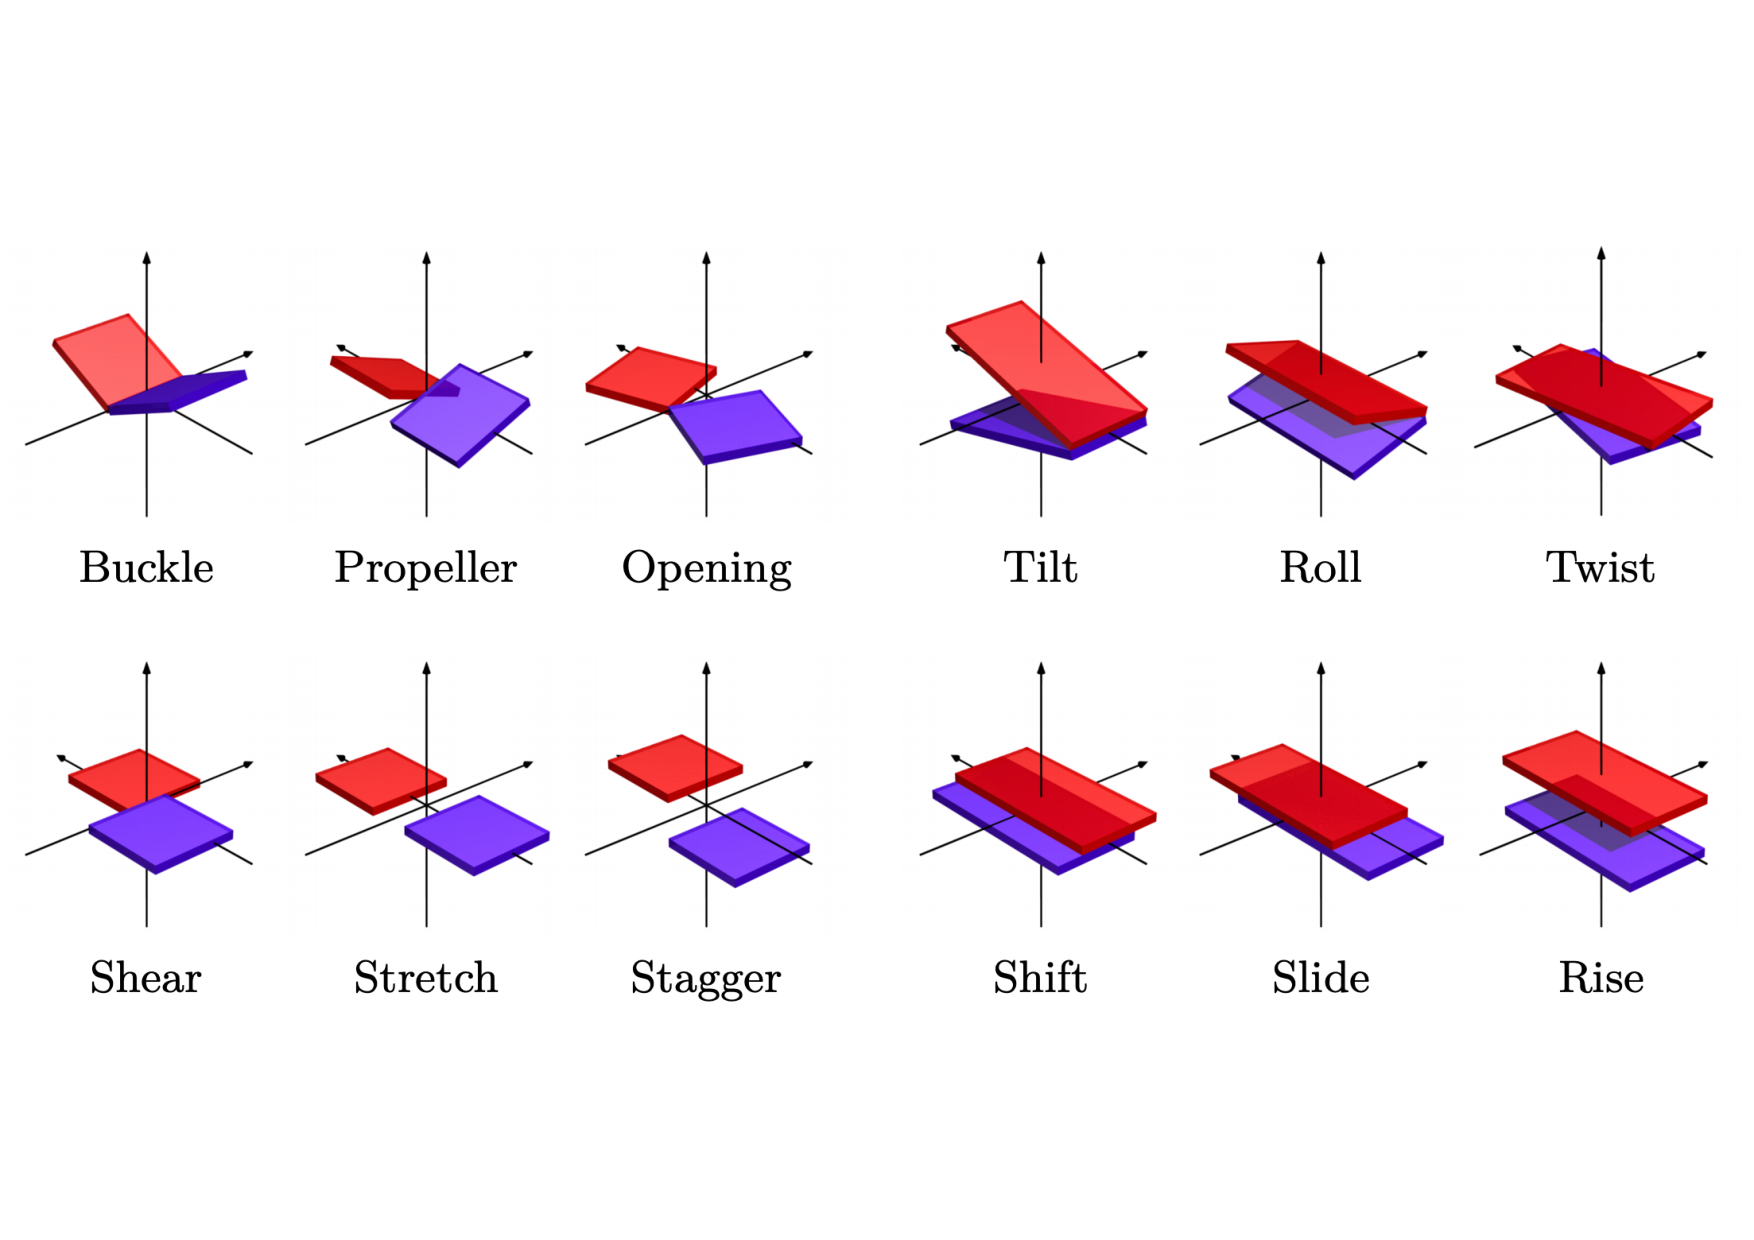
\includegraphics[scale=0.3]{./Xray_images/IC.pdf}
% 	\centering\caption{CURVES$+$ coordinates for a coarse-grained DNA configuration. Intra base-pair (left) and Inter base-pair (right). Image taken from~\cite{petthesis}.}
% \label{fig:IC}
% \end{center}
% \end{figure}

% \subsection{cgNA$+$ model}
% The cgNA$+$ model is a predictive model that given a
% sequence $\sq$ along the reading strand and a
% parameter set $\mathcal{P}$ delivers a Gaussian pdf in configuration space by reconstructing
% a ground-state $\hat{w} (\sq, \mathcal{P}) \in \R^{24N-18}$,
% and a positive-definite stiffness matrix $\K (\sq, \mathcal{P}) \in \R^{24N-18 \times 24N-18}$:

% \begin{equation}
% \rho(w; \sq, \mathcal{P}) = \frac{1}{\textit{Z}} exp \{-\frac{1}{2}(w-\hat{w})\cdot \K (w-\hat{w})\}.
% \label{c3:eq8}
% \end{equation}

% In cgNA$+$~\cite{patelithesis}, a parameter set $\mathcal{P}$ for DNA in its
% standard alphabet is made up of a) ten
% independent interior dinucleotide-dependent $\K^{\XY}$ 
% blocks $\in \R^{42 \times 42}$ plus sixteen
% independent $\K^{5'\XY}$ end blocks
% $\in \R^{36 \times 36}$, and b) ten independent interior dinucleotide-dependent stress vectors
% $\sigma^{\XY} \in \R^{42} $ plus sixteen independent $\sigma^{5'\XY}$ end stress vectors
% $\in \R^{36}$,
% \begin{equation}
% \mathcal{P} = \{ \sigma^{5'\XY},  \sigma^{\XY}, \K^{5'\XY}, \K^{\XY} \} \in
% \P = [\R^{36}]^{16} \times [\R^{42}]^{10} \times [\R^{36 \times 36}]^{16} \times [\R^{42 \times 42}]^{10}
% \label{eq:eq2}
% \end{equation}
% where $5'\XY \in\{16$ end dimer steps$\}$  and
% $\XY \in\{10$ independent dimer steps$\}$. The parameter for $3'$
% ends and dependent dimer steps can be obtained using Crick-Watson (CW) symmetry.

% One of the most important feature of the cgDNA family of models is that the
% $\K$ matrix and $\sigma$ vector have local sequence
% dependence (nearest-neighbors only) but the
% ground-state configuration which is given as:
% \begin{equation}
% \hat{w}(\sq) = \K^{-1}(\sq)\sigma(\sq)
% \label{eq:eq3}
% \end{equation}
% has non-local (often strongly non-local) sequence
% dependence because of the matrix inversion which
% reflects the physical phenomenon of frustration (only possible in
% double chain rigid base model or higher hierarchy models like cgNA$+$).

% The cgNA$+$ parameter set has been trained on long-scale MD time-series for a library of palindromic sequences~\cite{patelithesis}. All the simulations 
% were performed using AMBER 18 modules~\cite{amber}
%  using the BSC1 (parmbsc1)~\cite{parmbsc1} forcefield in explicit TIP3P~\cite{tip3p} water and 0.15M K$^{+}$,Cl$^{-} \;$ Joung-Cheatham ions~\cite{jcion}.
% More details on the MD protocol can be found in ref.~\cite{patelithesis}. \rs{cite the manuscript which will be prepared later}

\subsection{Database definition}\label{Database}
Protein-DNA X-ray crystal structures have been taken from the RCSB Protein Data Bank~\cite{berman2002protein} (www.rcsb.org) (last updated here in August 2020) using Biojava~\cite{biojava,biojava5} for retrieval and caching, and for implementing the criteria to identify redundant structures.
Since some of the protein-DNA crystal entries in this database include identical sequences bound to the same protein or nearly the same protein with small chemical changes (examples include nucleosome structures with an identical 147 bp DNA sequence bound to histone core protein, such as structures with PDB accession codes 1KX5, 5AV5, 5AV6, 5AV8, 5AVA, 5AVB, and 5AV9), which can bias the statistics, we developed and implemented a method to identify redundant structures. 

%The different sequences bound to the same protein do provide new information about the compatible flexibility of such sequences as the induced bending should be different for different sequences due to aspects like different hydrogen-bonding patterns with the protein; however, the inclusion of the same sequence multiple times would bias the statistics towards certain protein-induced bending modes.
%Providing a nearly random sampling of proteins for each tetramer is necessary to develop an X-ray model from a uniform exploration of the DNA conformational space. %\rs{details provided by Luke, some parts may go to SI}

The different sequences bound to the same protein do provide new information about the compatible flexibility as the induced bending is different for different sequences due to aspects like different hydrogen-bonding patterns with the protein; however, the inclusion of the same sequence several times would bias the statistics toward certain protein-induced bending modes. 
Therefore, such redundant structures must be discarded to explore the unbiased dsDNA conformational space.
To identify redundant information, which would involve the same sequence or nearly an identical sequence bound to the same protein, ECOD (evolutionary classifications of domains)~\cite{ecod} classification groups are used to identify the protein category, and then sequence matching (having a longest common sub-sequence in two structures that is greater than 70 \% of the total DNA length) is used as the second criterion to determine if a structure is redundant compared to one previously chosen if it is bound to the same protein. For structures that meet both criteria, the one with the better X-ray resolution is chosen, and the other structures that are nearly identical in sequence and bound to the same protein are discarded.

Subsequently, we have coarse-grained those selected atomistic structures by fitting a rigid-body frame~\cite{svdfit} using standard DNA atomic coordinates defined in the Tsukuba convention~\cite{tsukuba}. From these frames, we obtained 
 CURVES$+$ internal coordinates~\cite{curveplus}. Lastly, from a sequence of any length, we have extracted coordinates of all dimers in their tetramer contexts with the constraint that the tetramer should be at least two base-pairs away from ends.

\begin{figure}[htb!]
	\begin{center}
	\centering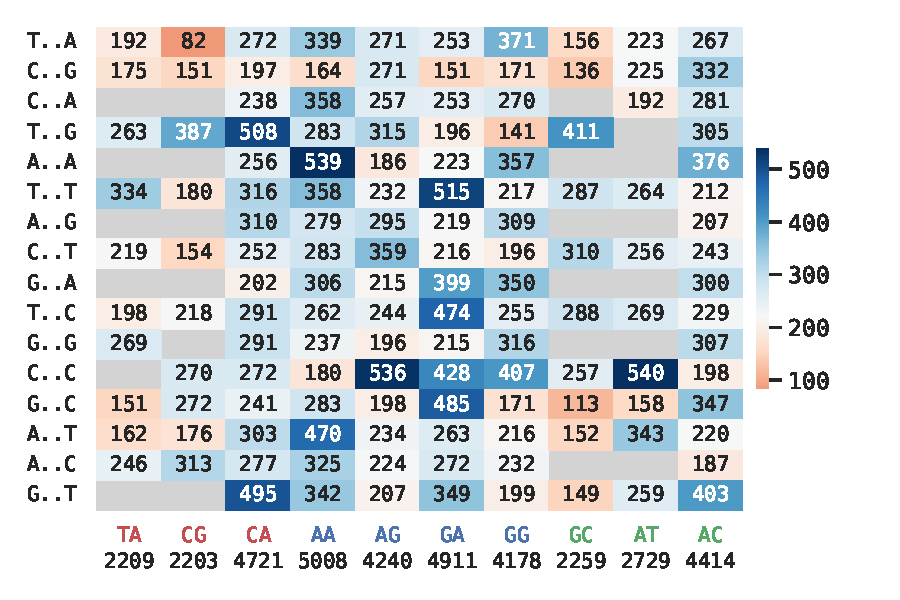
\includegraphics[scale=1]{./Xray_images/freq_heat_map_tt3_3S_C1_cg_unsym.pdf}
	\centering\caption{
	Number of appearances of 136 independent tetramers in X-ray data set (case-\Rom{1}). Abscissa is middle junction dimer-step and ordinate is flanking tetramer context. The blank entries in the plot represent the dependent tetramer. Note that palindromic steps (self-complementary) are only read from the reading strand here. Further note that while computing the sequence-independent average and covariance, we consider all 256 tetramers and for palindromic steps, we have used double of their corresponding weights (details in \cref{ss:avg_cov}).
%\rs{explain ....}
}
\label{fig:freq}
\end{center}
\end{figure}
\color{black}

Furthermore, the crude data contain some entries with highly distorted DNA, broken H-bonds, and nicks which requires filtering. 
One of the consequences of these distortions is that the rotation angles may go very close to $\pi$. 
In cgNA$+$ coordinates, rotation angles are defined as the norm of Cayley vector~\cite{petthesis,patelithesis} which tends to infinity when the angle approaches $\pi$ (details in \cref{c2:fra_to_int}).
It allows us to efficiently filter such cases as the corresponding Cayley components become very high (of the order $\sim 10^6$). 
This step removed $\approx 9\%$ of the data.
Following this, to ensure that each parameter follows a 
quasi-normal distribution and does not have long asymmetric tails, we adopted a variant of the $3\sigma$ method
used originally in ref.~\cite{xraydata}. We remove a snapshot if any parameters are outside three standard deviations from the mean. 
This method has been often used to curate X-ray data~\cite{xraydata,perez2004relative}, but only while using inter parameters and at the dimer level, which allows the algorithm to converge in 5-6 steps.
However, in our case, we are using 18 parameters and analyzing 136 tetramers, which rejects $\approx 50 \%$ of the data and convergence requires 10-20 cycles.
An alternative approach might be to reject the dimer steps that have broken H-bonds~\cite{fujii2007sequence}, but with a risk of long tails in the distribution of some of the internal coordinates for some of the tetramers.
Therefore, in this chapter, we decided to use the $3\sigma$ approach for just one cycle (to eliminate long asymmetric tails, if any) and ensure that the accepted data contains no broken H-bonds keeping $\approx 70 \%$ of the crude data.
Moreover, we also analyzed the data obtained after two and three cycles of the above
approach and found a negligible impact on the conclusions as it only removes the data from the tails without influencing the mean.


Lastly, we performed our analysis for two sets of data \Rom{1}) No resolution cut-off on PDB structures and \Rom{2}) PDB structures with at least 3.0 \AA \; resolution or better. 
In the chapter, we have presented results for case-\Rom{1} and for case-\Rom{2}, corresponding results are provided in \cref{app5}.
The precise number of instances for each tetramer in the X-ray data set for case-\Rom{1} and case-\Rom{2} are provided in \cref{fig:freq,SIfig:freq}, respectively.

\subsection{Methods to compare X-ray statistics with cgNA$+$ statistics}
%\rs{explain this section better, explain better the mu* and other technical things}
\subsubsection{Computation of sequence-independent groundstate and covariance}\label{ss:avg_cov}
To compute the sequence-independent (or sequence-average) groundstate and covariance, we have considered all 256 tetramers with double the corresponding weights for palindromic steps.
It is because, for non-palindromic steps, we are counting the same physical dimer step twice while reading from both the strands; therefore, to balance the statistics, we are taking double weights for the palindromic steps. 
In this chapter, we have defined two covariance matrices, namely, shape covariance ($C_s$) and configuration covariance ($C$) defined as: 
\begin{equation}
C_s=\frac{\sum_{i=1}^N w_i \left(x_i - \mu^*\right)\left(x_i - \mu^*\right)^T}{\sum_{i=1}^{N}w_i}
\text{ where } \mathbf{\mu^*}=\frac{\sum_{i=1}^N w_i x_i}{\sum_{i=1}^N w_i}
\end{equation}
\begin{equation}
C=\frac{\sum_{i=1}^N w_i \left(C_i + x_ix_i^T  \right)}{\sum_{i=1}^{N}w_i} - \mu^*(\mu^*)^T
\end{equation}
where $w_i$, $x_i$, $C_i$, and $\mu^*$ are the weight (or number of instances), average shape, covariance for a given tetramer, and weighted sequence-independent (i.e., sequence-average) average shape, respectively.
Shape covariance ($C_s$) is computed over the groundstate of dimer in tetramer context and
can be described as the directions in which groundstate varies over sequence space. 
For the X-ray data set, configuration covariance ($C$) is defined as the deformation of DNA in the configuration space computed over all entries in the X-ray data set. 
For cgNA$+$ model data set, it is the Gaussian average of the covariance matrices for DNA dimer in tetramer contexts.
We would like to emphasize that the groundstate and covariance computed using 256 tetramers will respect the palindromic properties as discussed in \cref{ss:parity}.  
Note that we have used the subscript $X$ and $M$ to highlight the statistics from the X-ray and cgNA$+$ model data sets, respectively. 
For instance, $C_s^X \and C_s^M$ are shape covariance for  X-ray and cgNA$+$ model data sets, respectively.


\subsubsection{Eigenvector parity}\label{ss:parity}
There is an inherent CW symmetry in the groundstate of dsDNA due to the reading strand choice. 
$E$ ($= E^T$) matrix (reading strand transformation matrix defined in \cref{c2:sec3sb1}) maps the groundstate of dsDNA read from one strand to another, i.e., $\mu(\bar{S})=E\mu (S)$. 
This inherent CW symmetry is also reflected in the configuration covariance matrices and thus, follows the CW symmetry condition $C(\bar{S})= EC(S)E$.
For a palindromic or self-complementary sequence (invariant of reading strand) or the average sequence (which is also invariant of reading strand), $S=\bar{S}$, the relation becomes $\mu(\bar{S})=\mu (S)$ and $C(S)= EC(S)E$. 
For such palindromic cases,
\begin{equation}
    D = P^TCP = P^TECEP = (EP)^TC(EP)
\end{equation}
where $D$ and $P$ are the eigenvalue (eigenvalues on the diagonal) and eigenvector matrix (with columns as eigenvector), respectively. 
Due to CW symmetry, if $P_i$ is an eigenvector, then $EP_i$ is also an eigenvector with the relation $P_i=\pm EP_i$ where positive or negative signs define a parity of the eigenvector.
Furthermore, we used cosine similarity to compare eigenvectors in the two covariance matrices, defined as the dot product ($P_i \cdot P_j$) between the corresponding eigenvectors.
Note that we have continued to use the subscript $X$ and $M$ to highlight the statistics from the X-ray and cgNA$+$ model data sets, respectively. 

\subsubsection{Hierarchical Clustering}\label{ss:cluster}
Clustering is an unsupervised machine learning method that finds patterns in the data sets consisting of input data without labels. 
It finds meaningful structure, features, and groupings inherent in the input data.
In particular, we have performed hierarchical clustering (which group data into a tree of clusters) on the groundstate of dsDNA dimers in tetramer context using the square root of symmetric Mahalanobis distance, $\M$ (defined in \cref{a3:eq13}) as the metric and average linkage as the linkage algorithm~\cite{clustering_muller}.
The standard python or Matlab linkage algorithm is used in which the distance $\D(p,q)$ between two clusters is computed. 
The algorithm starts by treating every data point as an individual cluster and then 
combining two nearest clusters, say $p$ and $q$, into one cluster, and then removing $p$ and $q$.
It iterates until only one cluster is left, which becomes the root. 
The average linkage algorithm defines the distance between two clusters as 
\begin{equation}
\D(p,q) = \frac{1}{|p|*|q|}\sum_{i=0,j=0}^{i=|p|,j=|q|} \sqrt{\M(\rho_i,\rho_j)}
\end{equation}
where $|p|$ and $|q|$ are cardinalities of clusters. \clearpage

\subsubsection{Configurational volume}\label{ss:con_vol}
For X-ray crystal data or atomistic simulations, the deformability of DNA can be quantified in terms of fluctuations of internal coordinates in the configuration space.
For fluctuations $\in \R^N$, configurational volume~\cite{xraydata,olson2006dna} can be defined as:
\begin{equation}
S = \sqrt{\lambda_1\lambda_2 \cdots \lambda_N}
\label{eq:eq2}
\end{equation}
where $\lambda_i$ are the eigenvalues of the covariance matrix, C $\in \R^{N \times N}$.
The unit of S is equivalent to $\text{\AA}^{N/2}\cdot(rad/5)^{N/2}$.

\subsection{Assumptions in this study}\label{ss:limitation}
\begin{itemize}
    \item The primary assumption in this comparison is that in protein-DNA X-ray crystal ensemble, distortions of dsDNA resulting from proteins effectively balance out for a sufficiently large ensemble exposing the intrinsic mechanical behavior of dsDNA. 
It leads to the following assumption that we have sufficient data for each dimer in the tetramer context. 
The exact number of instances for each dimer in the tetramer context is provided in \cref{fig:freq}. 
For most tetramer contexts, we have at least 150 instances (after filtering), and the distribution of internal coordinates is peaked around a particular 
value (sometimes bi-modal) providing confidence in the statistics, at least for the groundstate. 
Moreover, as described in \cref{ss:parity}, groundstate for the palindromic dimer should be invariant of the reading strand, which allows us to define the palindromic error (refer \cref{c2:s5sb1}) to quantify the convergence in X-ray statistics. 
For X-ray data set, palindromic error for dimer in tetramer context is $0.0197$ while for dimer in average tetramer context is $0.0042$ (details in \cref{SIfig:palin_error}).
Notably, the corresponding palindromic error in MD simulations training data for the cgNA$+$ model is $0.0025$ and 
$0.00037$, respectively, which contains $\sim 10^7$ snapshots. 
%\rs{wasnot clear to oliver} 
Even though the palindromic error is the norm of a scaled vector with mixed rotational and translational entries, \AA \ or rad/5 can be treated as the units of palindromic error.
The palindromic error obtained in the X-ray data set is still reasonable because, in the X-ray data set,  flanking sequence beyond
 tetramer context is different for most entries.
\item Furthermore, in this comparison, we have only considered the first and second moments of the distribution of helical internal coordinates for each dimer step (either in average context or tetramer context).
However, it is well known that for some of the internal coordinates, there exists an inherent bi-modality in helical internal 
coordinates~\cite{dans2012exploring}. 
Further investigation of bimodality is outside the scope of this chapter (also limited by the scarcity of experimental data) and was previously discussed at dimer level in ref.~\cite{olson2011working,dans2012exploring}.

\item Lastly, it is not clear how physical conditions in crystallization experiments 
(which might be different for each protein-DNA complex) influence the mechanics of dsDNA. 
For example, the effective temperature of protein-DNA crystal ensemble is significantly less than in
atomistic MD simulations and is unknown and not easy to determine~\cite{lankavs2003dna,becker2006indirect}. Furthermore, other factors such as divalent cations, salt concentration, buffer-type, and packing forces are poorly understood.
\end{itemize}

\section{Results and Discussion}
%In this section, we have compared the groundstate of 136 tetramers in 18 internal coordinates 
%which is not easy to comprehend using a traditional one-to-one comparison. Therefore,  
%we first compared the sequence-independent groundstate of dimer and then the direction of variation of groundstate over tetramer sequence space.  
%Furthermore, to quantify correlation between the groundstate of dimer in the two data sets, we have used linear 
%correlation as described in \cref{ss: cosine_sim}. 
%More details on one-to-one comparison of internal coordinates for the groundstate are provided 
%on the \rs{website}. 
%Lastly, to compare the stiffness or inverse configuration covariance, we have first compared the eigen-direction of sequence-average configuration covariance in the two data sets and then 
%used the measure of configurational volume as defined in \cref{ss:con_vol} to quantity and compare non-local sequence-dependent stiffness.

\subsection{cgNA$+$ model over atomistic MD simulations}
In the X-ray data set, each instance of a dimer in the tetramer context is most likely flanked by a different sequence.
However, it is not computationally feasible to perform atomistic MD simulations for tetramers in all the possible flanking sequences, even up to two base-pair steps on both sides.
In contrast, the cgNA$+$ model provides an excellent alternative whose predictions are almost indistinguishable from MD and can efficiently compute statistics for millions of sequences. 
In \cref{c4:figure1}, we have exemplified that the cgNA$+$ model prediction is almost indistinguishable from the corresponding MD statistics for a sequence outside the cgNA$+$ model training library.
Furthermore, in \cref{c4:figure1_rna}(b), we have also compared internal coordinates of middle junction dimers embedded in different beyond tetramer contexts for MD simulations and demonstrated that beyond tetramer context could influence the groundstate of junction dimer, and the cgNA$+$ model can capture such highly non-local changes due to change in hexamer or beyond context.
A detailed assessment of the cgNA$+$ model prediction accuracy is in \cref{c4}. 

Thus, in this chapter, we have used the cgNA$+$ model over MD simulations and reconstructed the groundstate and stiffness matrix of all possible sequences with a length of 10 base-pair steps (plus GC ends) using the cgNA$+$ model.
Subsequently, we extracted the marginal of the middle junction dimer in each tetramer context to obtain the statistics in the average flanking sequence context beyond tetramer context.

Lastly, we would like to remind that the cgNA$+$ model is a rigid-base and rigid-phosphate model which predicts the groundstate of a given sequence in base and phosphate internal coordinates.
However, in this chapter, we have only compared the cgNA$+$ model predictions with X-ray data set in base-coordinates (both intra- and inter-base coordinates) by taking marginals over the phosphate coordinates.
It is well known that phosphate coordinates are highly multi-modal (see \cref{c3:s6}) and is related to B\Rom{1}--B\Rom{2} backbone conformations~\cite{hartmann1993b,dans2019static} which is again found to be dependent on the sequence~\cite{dans2019static}.
Such comparison of backbone conformations in X-ray and MD data set was carried out previously in ref.~\cite{madhumalar2005sequence}.
Therefore, we believe that there are not enough experimental data to compare phosphates coordinates, particularly at the tetramer level, and is, therefore, left for further detailed investigations in the future.

\subsection{Comparison of groundstate}
%In this section, firstly,
%we have compared the sequence-independent 
% groundstate of dimer and directions in which
%the average-shape varies over the sequence space in the two data sets.
%Subsequently, we have compared the groundstate of dimers (in average flanking sequence) for
%cgNA$+$ model and X-ray data set. Following that, we have quantified how crucial is tetramer
%context for dimer groundstate. In the last subsection, we have compared the groundstate of
%dimer in tetramer contexts for cgNA$+$ model and X-ray data set.

\subsubsection{Comparison of dsDNA dimer groundstate and the directions of variations in groundstate over sequence space}
\label{ss:comp_avg_shape_direc}

\begin{figure}[htb!]
	\begin{center}
	\centering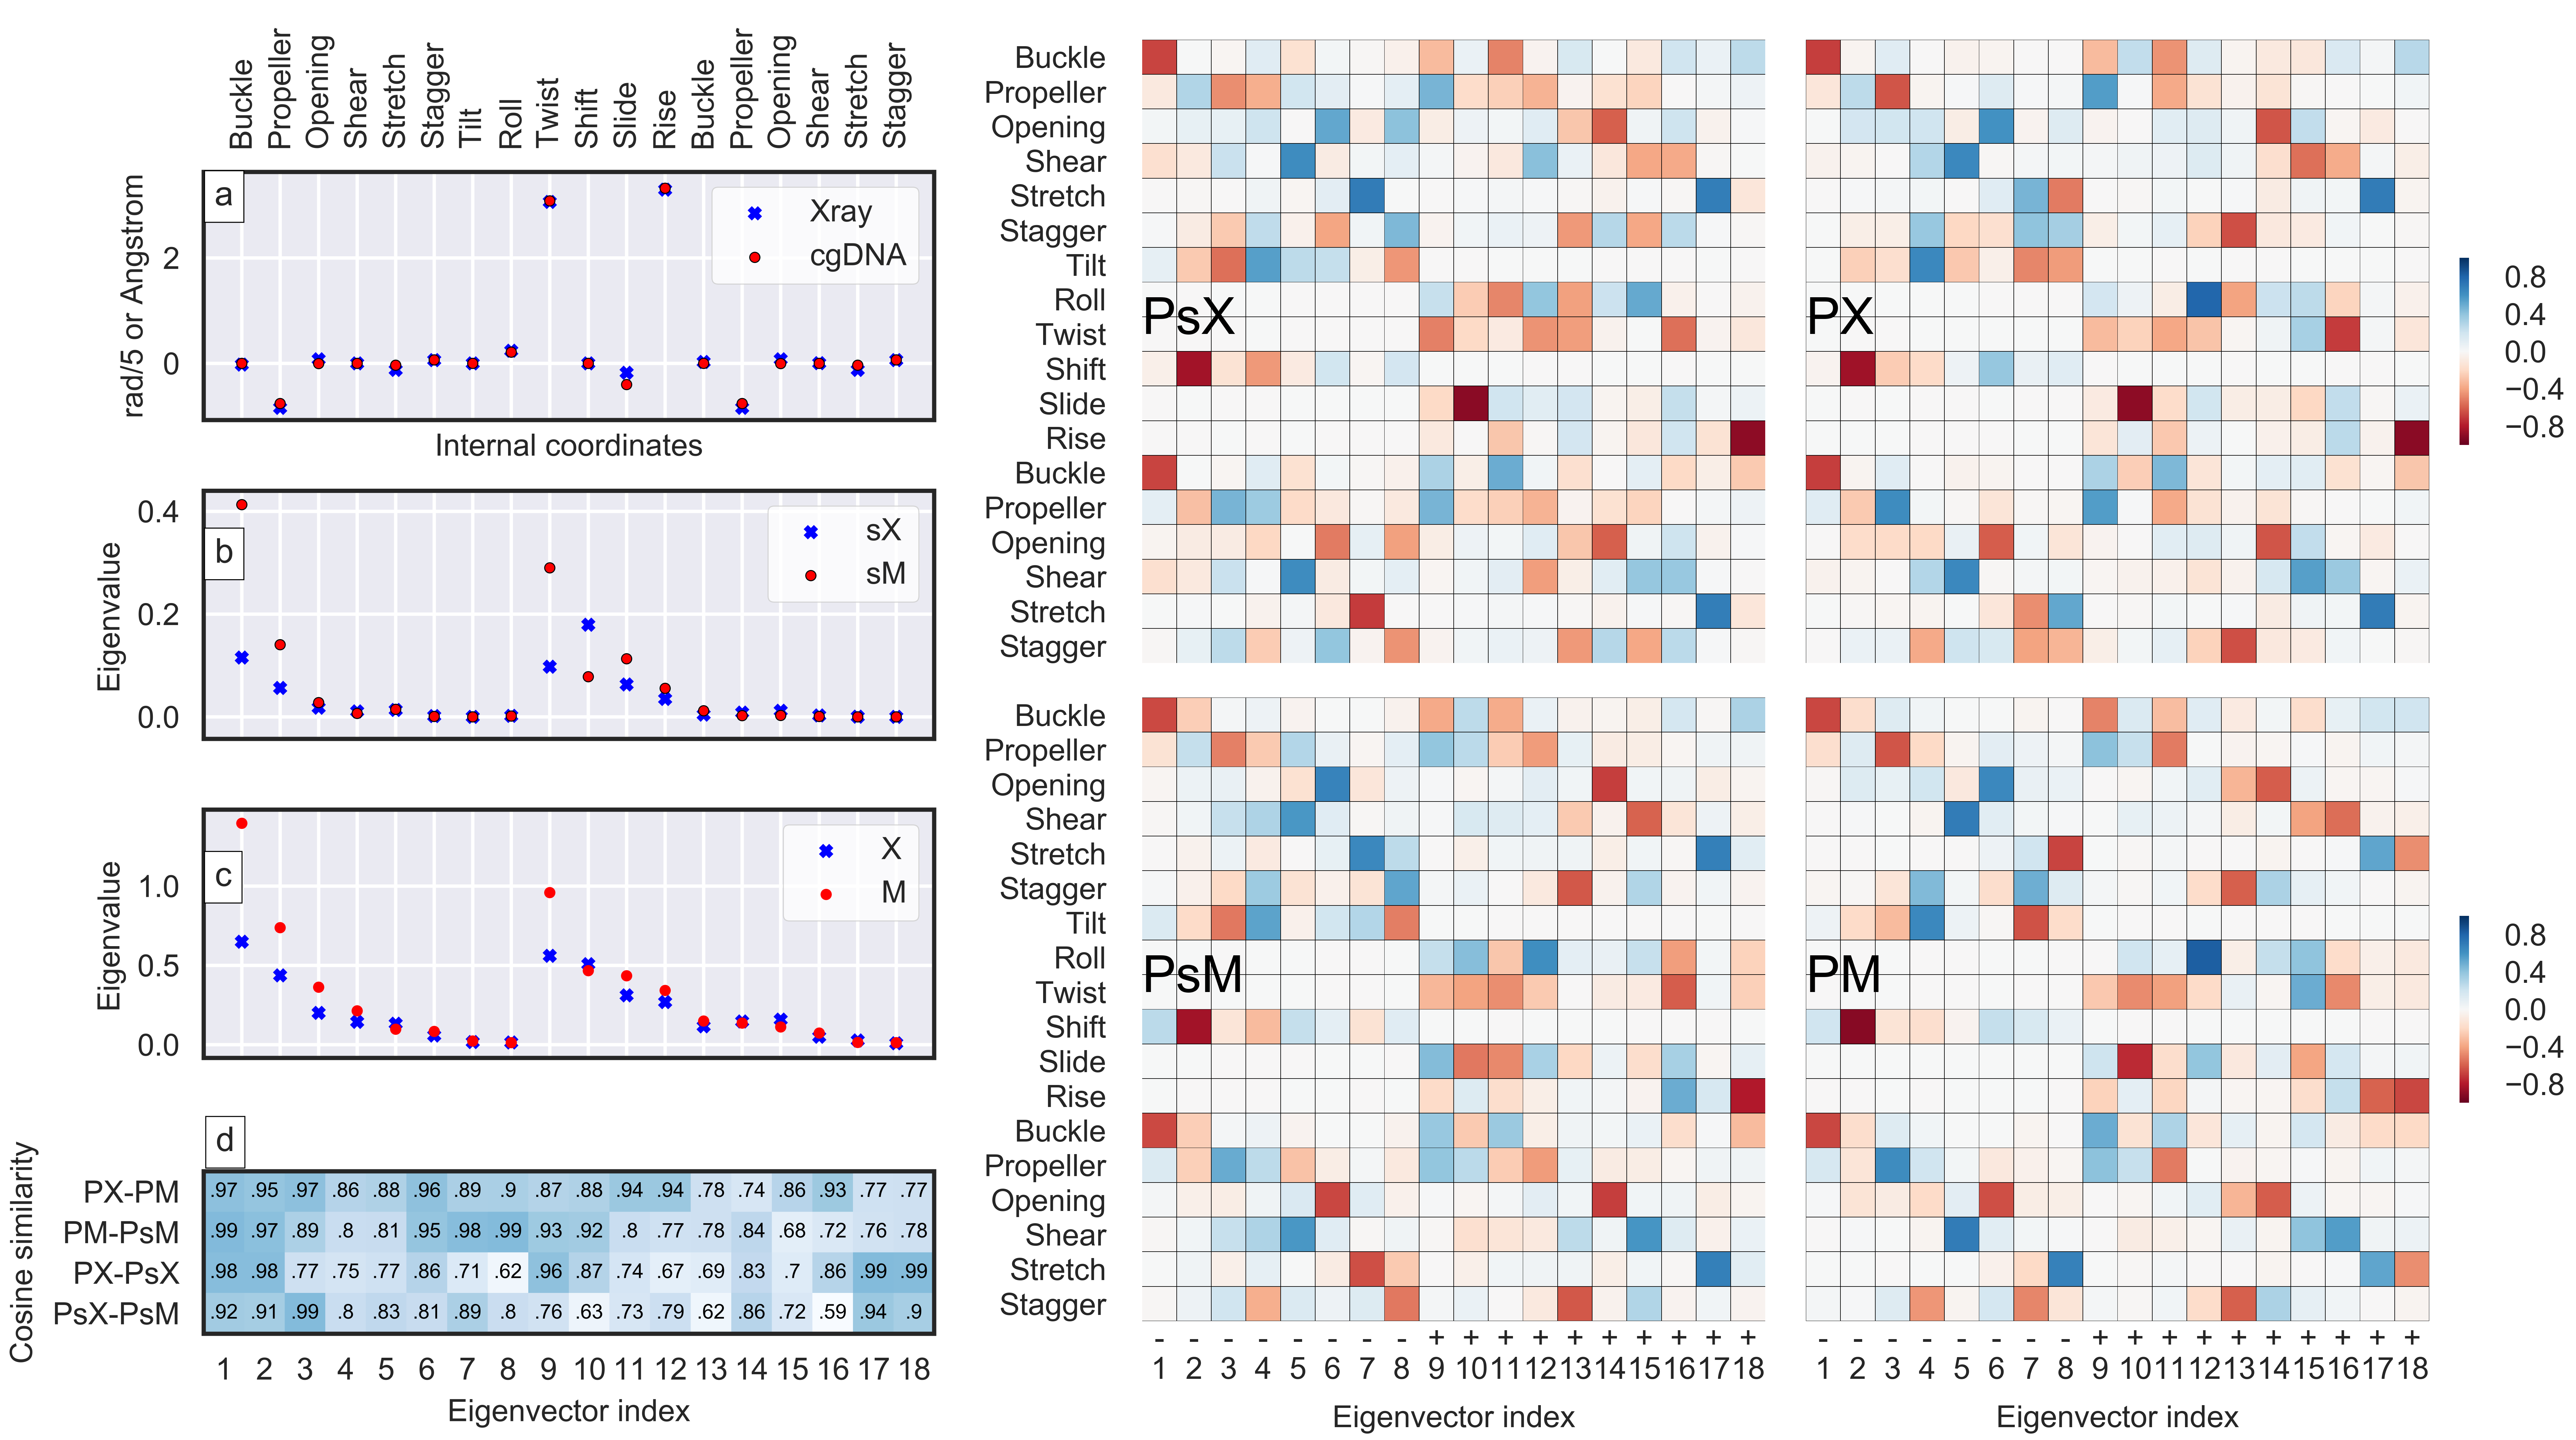
\includegraphics[scale=0.057]{./Xray_images/PP.png}
	\centering\caption{a) Plot comparing sequence-independent groundstate (average shape) of dimer coordinates in X-ray and cgNA$+$ model data set. On right, $P_s^X$ and $P_s^M$ are the associated eigenvector matrices for the shape covariance matrix (denoted by subscript s) describing the directions of variation in groundstate over sequence space for X-ray (denoted by superscript X) and cgNA$+$ model (denoted by superscript M) data sets, respectively and $D_s^X$ and $D_s^M$ are corresponding eigenvalues in b). While $P^X$ and $P^M$ are the eigenvectors of average configuration covariance 
	describing the direction of deformation of dsDNA in configuration space and $D^X$ and $D^M$ are corresponding eigenvalues in c). In d), there is cosine similarity index for corresponding eigenvectors in ($C^X,C^M$), ($C_s^M,C^M$), ($C_s^X,C^X$), and ($C_s^X,C_s^M$).  
	}
\label{fig:PMPX}
\end{center}
\end{figure}

In \cref{fig:PMPX}(a), firstly, we have plotted the sequence-independent (or sequence-average) average shape of the dimer predicted by the model along with the corresponding observations in the X-ray data set. The average shapes of dimers in the two data sets are very close.
These results agree well with previous findings~\cite{perez2008towards,fujii2007sequence,perez2004relative,olson2006dna,dans2012exploring,madhumalar2005sequence} limited to inter variables.

Furthermore, it is interesting to understand the directions in which groundstate of dsDNA varies over sequence space and whether these directions are consistent in the two data sets. 
We have computed \say{shape covariance matrices} denoted as $C_s^X$ and $C_s^M \in \R^{18 \times 18}$ for X-ray and cgNA$+$ model data sets, respectively, and plotted the corresponding eigenvectors ($P_s^X$ and $P_s^M$) and eigenvalues ($D_s^X$ and $D_s^M$) in \cref{fig:PMPX}.
The shape covariance matrices (defined in \cref{ss:avg_cov}) describe the directions in which groundstate varies over sequence space. 
$C_s^X$ and $C_s^M$ are shown in \cref{SIfig:cov_4} and ignoring the scale, the two matrices look very close and therefore, explored further by looking into the eigenvalues and eigenvectors.
For both the data sets, observed eigenvectors are quite sparse, in particular, follow a unique sparsity pattern with decoupling of inter variables with intra1 and intra2 variables (intra1 and intra2 are intra base-pair coordinates for the first and second base-pair of the dimer).
This decoupling originates from the inherent CW symmetry in groundstate of dimer and is algebraically explained in \cref{app4}.
There are 8 negative parity eigenvectors ($P_i=-EP_i$) with no fluctuations in the direction of Roll, Twist, Slide, and Rise, while for 10 positive parity eigenvectors ($P_i=+EP_i$), there are no fluctuations in the directions of Shift and Tilt where $P_i$ and $E$ are eigenvectors and reading strand transformation matrix. 
More details on reading strand transformation and eigenvector parity are provided in \cref{ss:parity}.
The number of positive and negative parity eigenvectors and this sparsity pattern in eigenvectors can be explained by inherent CW symmetry in groundstate of dsDNA. 
Now, the question arises how much eigendirections in the two data sets align? 
To quantify this, we have computed the cosine similarity (details in \cref{ss:parity}) between the best aligned eigenvectors in the two data sets which is plotted in \cref{fig:PMPX}(d). 
The average cosine similarity between the eigendirections of two data sets is $0.81 \pm 0.11$.
More importantly, in the two data sets, eigenvectors align approximately according to the magnitude of the corresponding eigenvalues, i.e., eigenvectors with comparable eigenvalues in both the data sets align with each other.
However, note that the magnitude of eigenvalues for the model shape covariance $C_s^M$ is larger than the corresponding aligned eigenvalues for X-ray data set $C_s^X$, particularly the larger ones.
It indicates that even though the direction of variation in the average shape over sequence space is similar, the magnitude of variation in the X-ray data set is less, which can be attributed to lower effective temperature in the X-ray data set.

%Buckle, Propeller, and Shear in intra base-pair coordinates and Tilt, Roll, Twist, Shift, and Slide in inter coordinates.
Another interesting observation is to identify the directions (in CURVES$+$ coordinates) from which eigenvectors are composed of. 
For example, eigenvectors with large eigenvalues are dominated by the Buckle, Propeller, and Shear (intra variables). While in inter variables, Rise is associated with the eigenvector that has the smallest eigenvalue and the rest of the CURVES$+$ inter base-pair coordinates seems important.
For the CURVES$+$ coordinates associated with eigenvectors with the lowest eigenvalues, the variation over the sequence space is so low that it is almost impossible to distinguish the sequence effect from the underlying noise.
This can be quantified by looking at the variance of internal coordinates for groundstates over sequence space as listed in \cref{tab:var_table}.
For example, the variance in Stretch and Rise over tetramer sequence space is $0.007$ and $0.006 \; \text{\AA}^2$ in X-ray data set. 
Notably, in the cgNA$+$ model data set, Stretch and Rise have relatively low variance than others.

\subsubsection{How crucial is tetramer context?}
In this section, we have investigated how crucial tetramer contexts are by comparing the dimers in specific tetramer contexts with those in the average context.
In \cref{fig:seq_imp2}, we have directly plotted the internal coordinates of a dimer in tetramer and average context as small and large horizontal lines, respectively, using a different color for each specific tetramer context and the last column as the sequence-average groundstate in each panel.
As can be seen in the plots, the internal coordinates of a dimer are, in general, sensitive to its context, and this sensitivity varies for different coordinates. 
In some cases, such as Buckle or Rise, the variation in groundstate due to flanking tetramer context change is larger than the variation in groundstate due to change in central dimer step in the average context.
Furthermore, the variation in some internal coordinates over sequence space is negligible, for instance, Stretch and Rise.
\Cref{fig:seq_imp2} contains all the data condensed into one plot to provide an overall picture of various aspects of the two data sets and for identifying exciting questions.
For instance, is there any pattern in dimer sequences (in average context) for which a given internal coordinate is far from the corresponding sequence-averaged internal coordinate or for a given dimer, which tetramer contexts result a dimer groundstate far from its groundstate in average context?
More standard questions include the correlation between the various internal coordinates in two data sets.
%\rs{more details on clustering in subsec}
%\rs{all the captions}

\begin{figure}[htb!]
	\begin{center}
	\centering\includegraphics[scale=1]{./Xray_images/seq_var_combine.png}
	\centering\caption{Plot of Intras and Inter for X-ray (bottom) and cgNA$+$ model (top) data set in which large dash lines depict internal coordinates of a dimer (in average context) while the other smaller dash lines are the internal coordinates for that dimer in a specific tetramer context. For better and concise visual representation, in each subplot, the three internal coordinates are slightly shifted on the X-axis. Also, separate flanking contexts are plotted in different colors as described at the bottom of the plot. SA is sequence-average groundstate.
	}
\label{fig:seq_imp2}
\end{center}
\end{figure}


Firstly, we have plotted the shifted (by the sequence-average shape) average shape for all the dimers in \cref{fig:logo_bits}(a) to visualize which dimers have the shape farthest or nearest to the sequence-average shape.
Once again, it can be observed that the spread of various internal coordinates is smaller in X-ray data than in the model data.
Furthermore, different dimer steps adopt extreme values for different internal coordinates.
For instance, RR and YY steps adopt the extreme values for Tilt and Shift, whereas RY and YR for Roll and Slide, and this trend is generally present in both data sets. 
In contrast, there is no clear pattern for Twist and Rise.

Moreover, from \cref{fig:seq_imp2}, it is clear that the flanking tetramer context significantly influences the average shape adopted by a dimer.
In \cref{fig:logo_bits}(b), we have attempted to answer which flanking contexts influence the shape of dimers the most. 
For each internal coordinate (IC), we have defined 
$\gamma_{\text{XUVZ}}= \text{IC}_{\text{XUVZ}} - \text{IC}_{\text{X}_{\text{avg}}\text{UV}\text{Z}_{\text{avg}}}$ as the difference of the internal coordinate of a dimer (UV) in tetramer context (X\,-\,-\,Z) with the same dimer in average context, where X, U, V, Z $\in$ [A, T, C, G]. 
Then, for each internal coordinate, we have defined positive and negative outliers as, $ \gamma_{\text{XUVZ}} < -\sigma$
and $ \gamma_{\text{XUVZ}} > +\sigma$, 
where $\sigma$ is standard deviation of $\gamma_{\text{XUVZ}}$.
In \cref{fig:logo_bits}(b), we have sequence logos plot with the information content in the tetramer flanking context (X\,-\,-\,Z) for which $\gamma_{\text{XUVZ}}$ are negative or positive outliers.
%Sequence logos are excellent graphical tools for visualizing and comprehending the underlying sequence pattern for any observables.
%In sequence logos, the x-axis is the base index in the sequences, and the y-axis is information content with the maximum possible value of two for NAs.
%The total height of the stack of A/T/C/G alphabets tells the information present in that index, and the relative height of alphabets represents their frequency at that index. 
Sequence logos are described in more detail in \cref{c1:sec_seq_logo}. 
From the sequence logos, it can be observed that dimer adopts extreme values only in specific flanking contexts. 
For instance, in the presence of Y\,-\,-\,Y flanking contexts, Tilt and Shift adopt a lower value than the average context, and the converse is true for R\,-\,-\,R flanking contexts.
Similarly, R\,-\,-\,Y and Y\,-\,-\,R flanking contexts tend to decrease and increase the equilibrium Slide values adopted by dimers, whereas the same contexts increase and decrease the equilibrium Twist and Rise values. 
Lastly, C/G flanking contexts decrease the equilibrium Roll values preferred by dimers, whereas A/T contexts have the opposite effect.
These observations are made for the cgNA$+$ model data set, but similar conclusions can also be made for X-ray data sets. 
In general, less information is present for the X-ray data set, which implies that the preference for particular flanking contexts is not equally strong. 
Moreover, for Roll and Shift, no information in flanking contexts. 
Note that the statistics are obtained for a limited X-ray data set, which might be noisy, so such an agreement is still impressive.
Thus, it can be concluded from the two subplots in \cref{fig:logo_bits} that different sequences prefer different equilibrium shape, and some conclusions can be made about their preference based on the pyrimidine or purine nature of the sequence.

An alternate way of exploring the role of tetramer contexts can be dendrograms using hierarchical clustering in the two data sets as plotted in \cref{fig:cluster}.
For clustering, we have used the square root of symmetric Mahalanobis distance~\cite{mahal} as the distance metric, and \say{average linkage} algorithm to compute the distance between clusters, which is defined in terms of the square root of Mahalanobis distance. More technical details on the dendrograms are provided in \cref{ss:cluster}.
In \cref{fig:cluster}, we observed similar clustering in both data sets, 
\begin{itemize}
\item there are three main clusters corresponding to YR, RR, and RY dimer steps with an exception in RR and RY clusters, where R is Purine and Y is Pyrimidine base. This classification highlights the importance of the middle-junction dimer step;
\item in each cluster, there are sub-clusters that correspond to the same middle junction dimer-steps in different
tetramer contexts. However, sub-clusters in YR cluster are not well-resolved; 
\item YR step is farthest from all the clusters (interestingly, YR dimer steps are found to be exceptionally flexible~\cite{xraydata}).
\end{itemize}

\begin{figure}
	\begin{center}
	\centering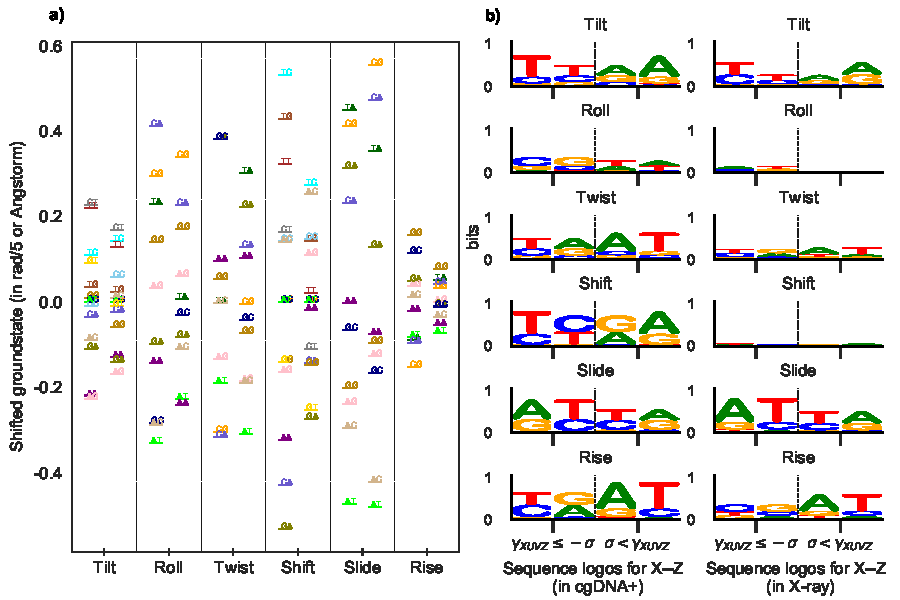
\includegraphics[scale=1]{./Xray_images/X3_logo_inter_mono-flank_bits.pdf}
	\centering\caption{
a) Inter coordinates (shifted with respect to sequence-average groundstate) are plotted for dimers in average flanking context to identify which dimers assume distant values from sequence-average groundstate for a given variable and whether that signal is consistent in the two data sets. 
For each IC, the left column is for the cgNA$+$ model data set and the right column is for the X-ray data set. 
b) Sequence logos plot to statistically quantify the role of tetramer context on the groundstate (in inter variables) of a given dimer.
For each internal coordinate (IC), we have defined $\gamma_{\text{XUVZ}}= \text{IC}_{\text{XUVZ}} - \text{IC}_{\text{X}_{\text{avg}}\text{UV}\text{Z}_{\text{avg}}}$ as the difference of the internal coordinate of a dimer (UV) in tetramer context (X\,-\,-\,Z) with the same dimer in average context, where X, U, V, Z $\in$ [A, T, C, G]. 
Then, for each internal coordinate, we have defined positive and negative outliers as, $ \gamma_{\text{XUVZ}} < -\sigma$ and $ \gamma_{\text{XUVZ}} > +\sigma$, where $\sigma$ is standard deviation of $\gamma_{\text{XUVZ}}$.
In the sequence-logos plot, we have plotted the information content in the tetramer flanking context (X\,-\,-\,Z) for which $\gamma_{\text{XUVZ}}$ are negative or positive outliers.
}
\label{fig:logo_bits}
\end{center}
\end{figure}

%\rs{may discuss the bias in protein-DNA data}

\begin{figure}[htb!]
	\begin{center}
	\centering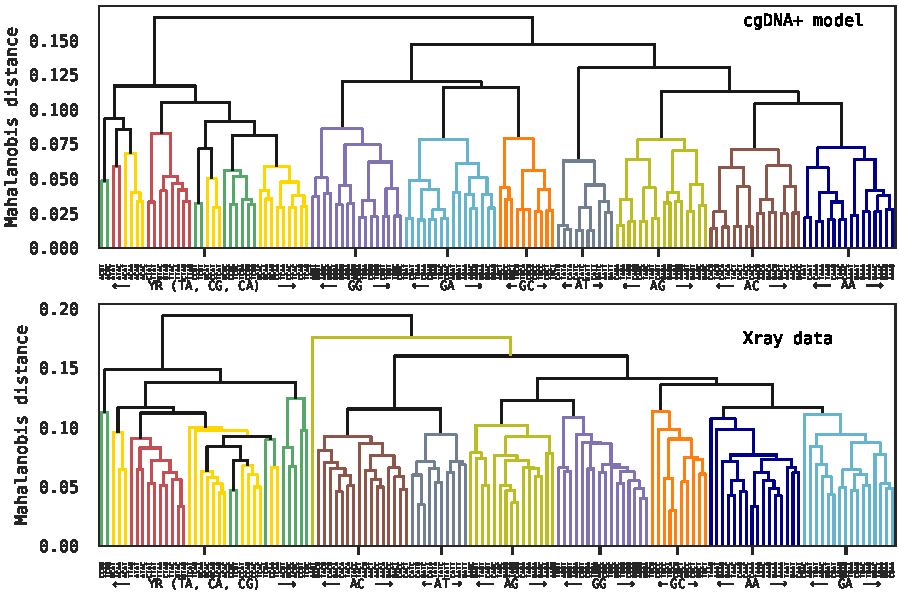
\includegraphics[scale=1]{./Xray_images/Dendrogram_cgxray_X3.pdf}
	\centering\caption{Dendrograms using hierarchical clustering on independent tetramers using square root of symmetric Mahalanobis distance (taking inverse of sequence-dependent configuration covariance as the weight matrix) as metric and average linkage algorithm \cref{ss:cluster}.
	%Note that the outliers in the dendrogram for the X-ray data set have a higher number of appearances in the X-ray crystal data base. Namely, TCGG (387), GCAT (495), CGAC (428), and TGCG (411). 
	}
\label{fig:cluster}
\end{center}
\end{figure}
%\vspace{-0.6cm}
\begin{figure}[htb!]
	\begin{center}
	\centering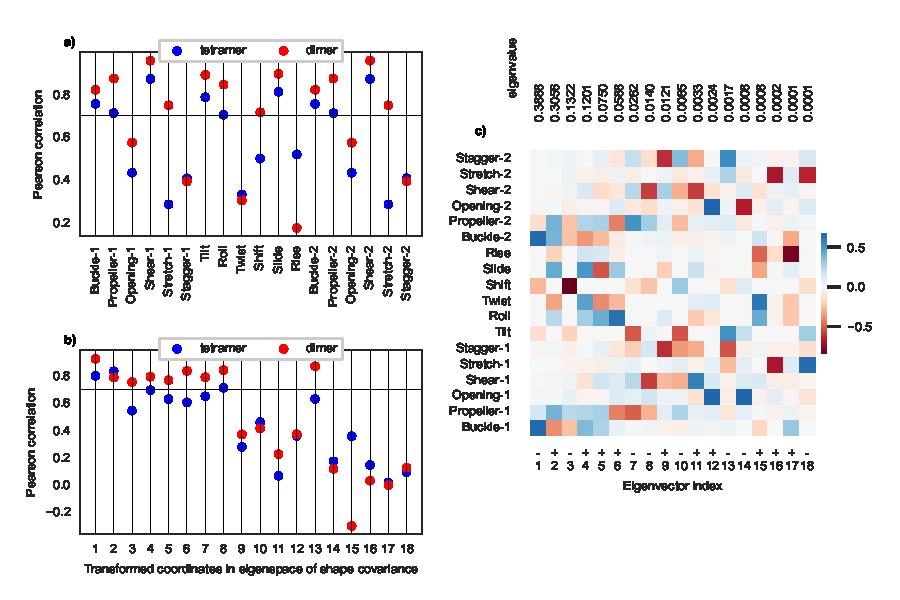
\includegraphics[scale=0.96]{./Xray_images/X3_CG_256_PC_one_one.pdf}
	\centering\caption{Pearson correlation between X-ray and cgNA$+$ data set a) in standard CURVES$+$ coordinates and b) in transformed coordinates in the eigenspace of cgNA$+$ shape covariance and the corresponding eigenvectors shown in c) with the $+/-$ parity as defined in \cref{ss:parity}.
	}
\label{fig:PC_one_one}
\end{center}
\end{figure}

At the same time, there are some differences in the dendrograms for the two data sets; notably, the distance between clusters is not the same in the two data sets, which can be attributed to the fact that the magnitude of shape covariance and configurational covariance in the two data sets are not identical due to lower effective temperature in X-ray data set.
With these observations, we can conclude that the tetramer context plays a crucial role in the dimer groundstate and thus, dimer models are not sufficient for a complete description of sequence-dependent mechanical properties of dsDNA. Therefore, in the next section, we have performed a further rigorous analysis comparing groundstate of dsDNA dimer in all independent tetramer contexts.

\begin{figure}[htb!]
	\begin{center}
	\centering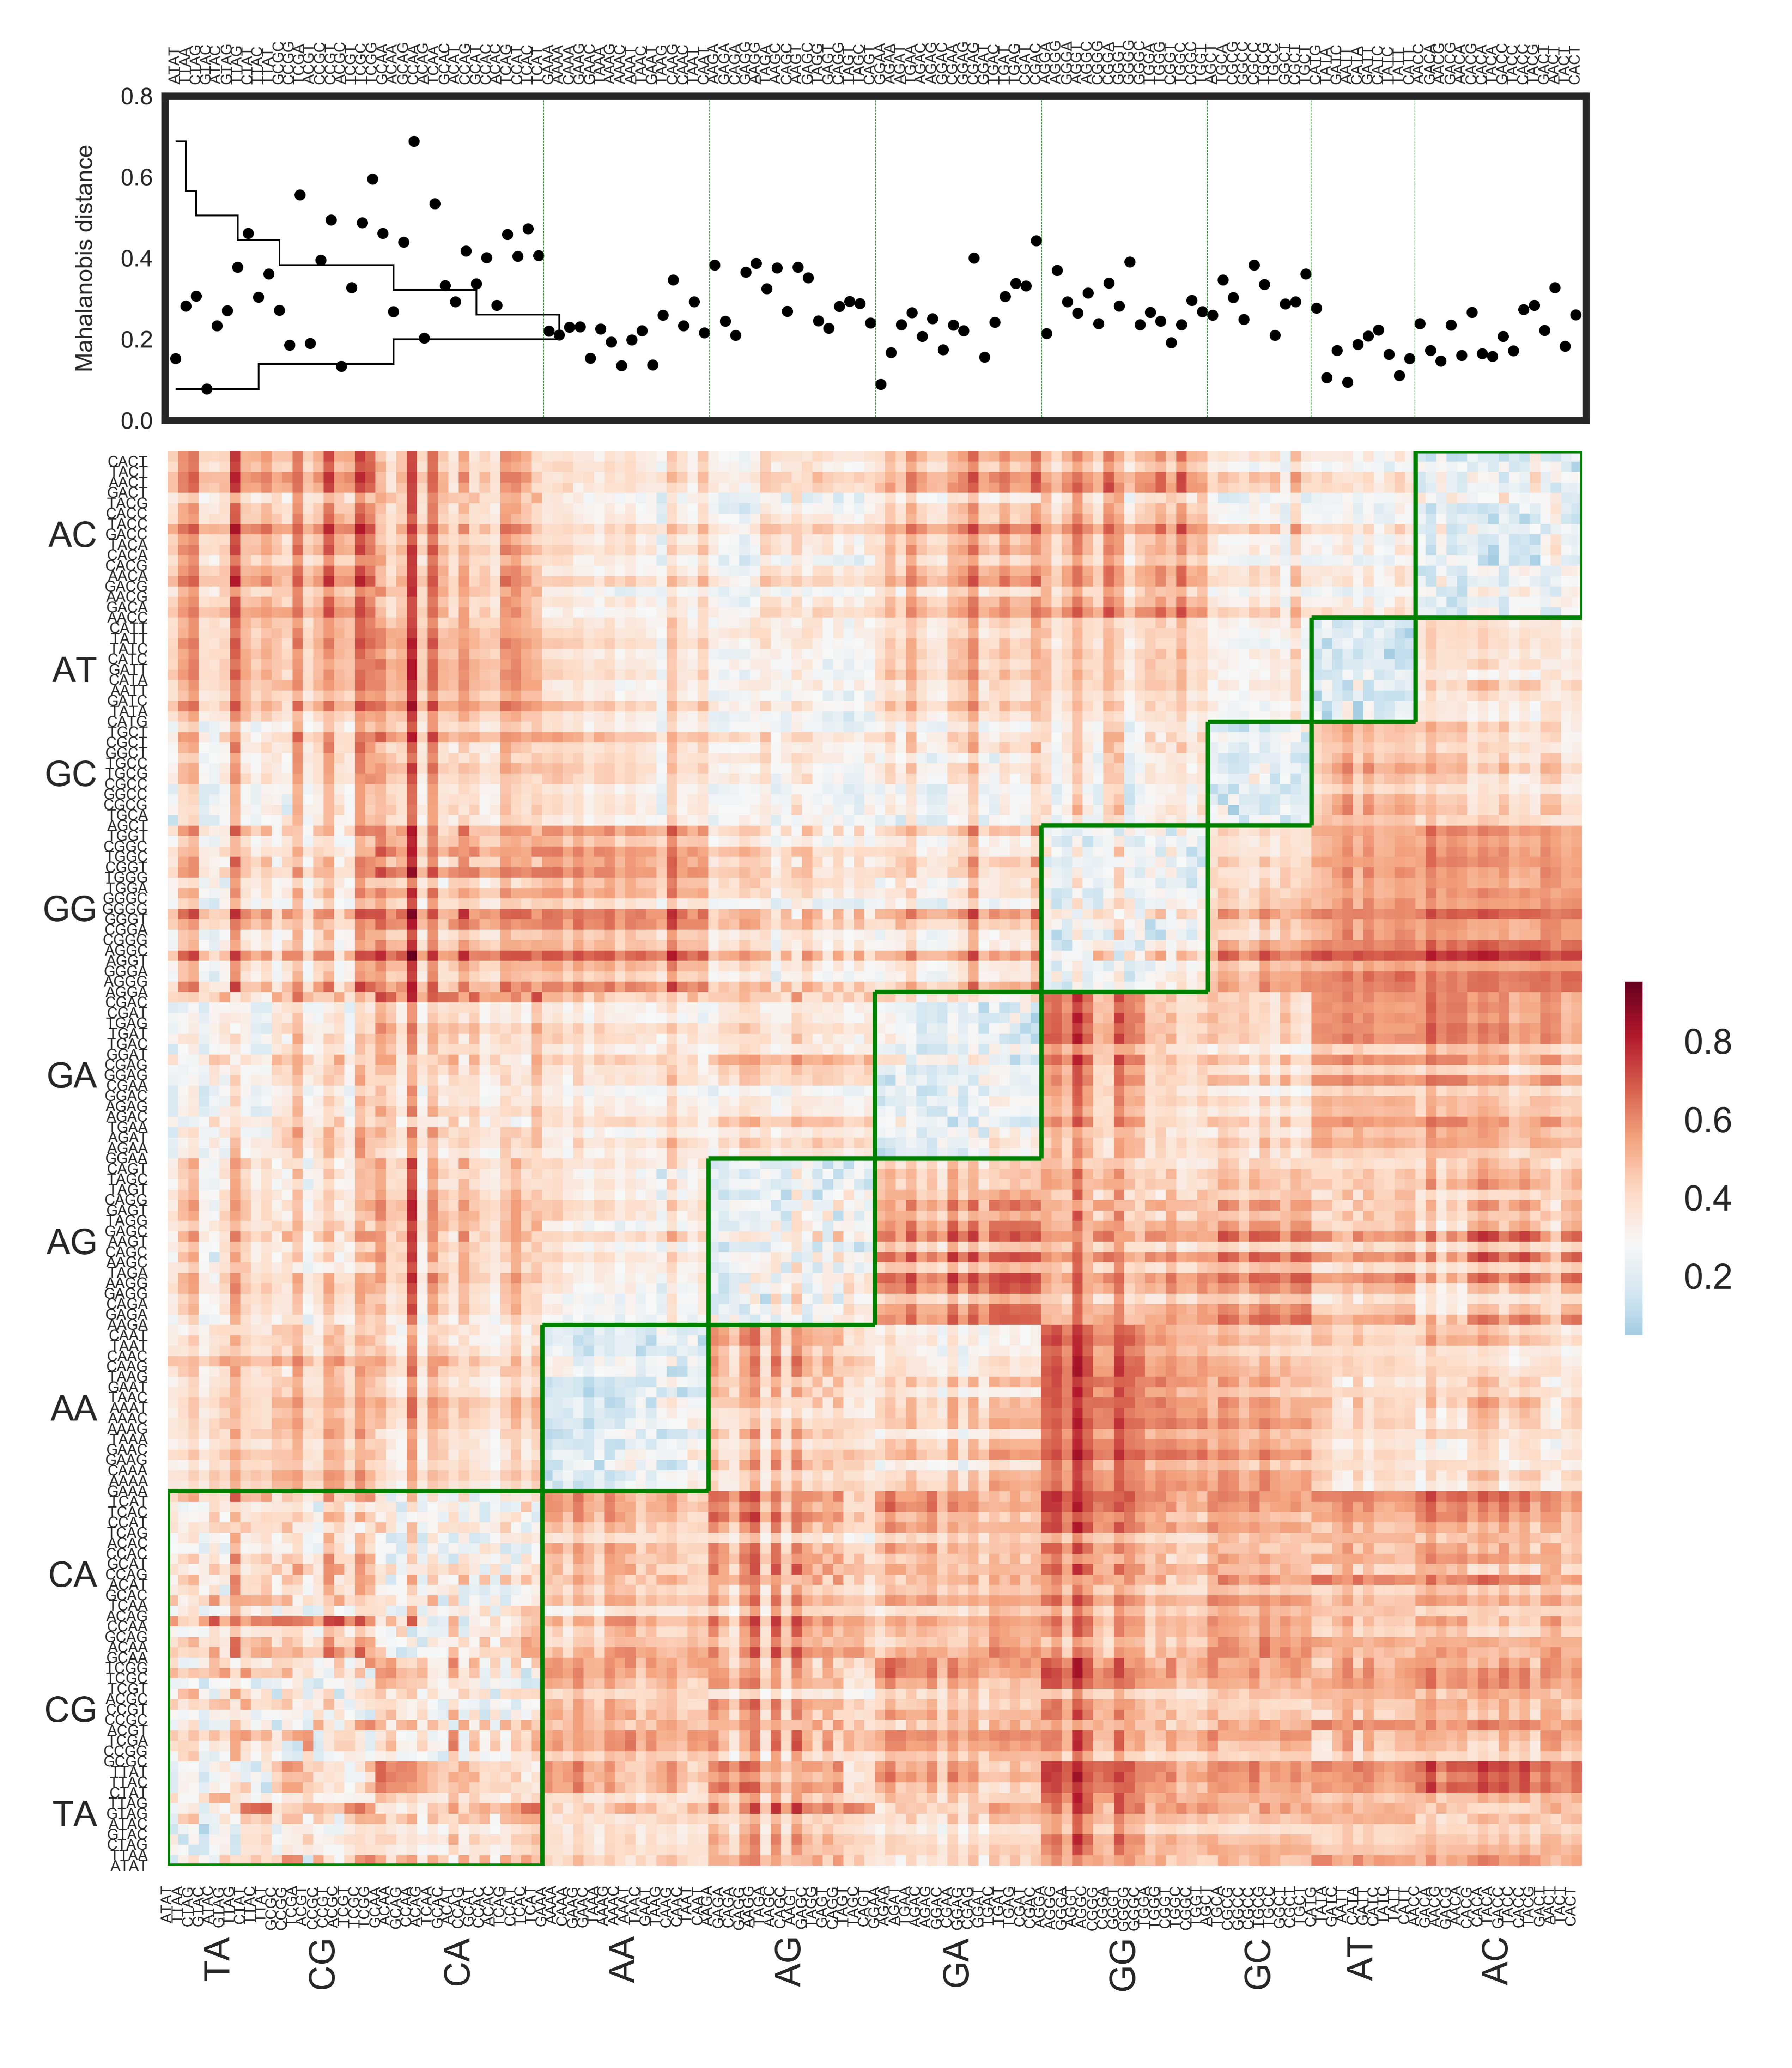
\includegraphics[scale=1.45]{./Xray_images/Mahal_comb.png}
	\centering\caption{
%	\rs{write clearly}
	In the heat map (bottom), the diagonal entries are Mahalanobis distance between the groundstate of dimers (in 136 independent tetramer contexts) in the X-ray and cgNA$+$ model data set. Whereas lower and upper off-diagonal entries are Mahalanobis distance between different dimers (in specific tetramer context) within the cgNA$+$ model and X-ray data set, respectively. The diagonal entries of the heat-map are again plotted in the scatter plot (top) along with the histogram in the same plot.
	Note that the Mahalanobis distance (defined in \cref{c2:s5sb3}) is computed in the transformed coordinates in the eight principal modes of cgNA$+$ shape covariance and using cgNA$+$ shape covariance matrix (in transformed coordinates) as the weight matrix. 
    The equivalent plot using all 18 CURVES$+$ coordinates is shown in \cref{SIfig:Mahal_18}.
	}
\label{fig:Mahal_8}
\end{center}
\end{figure}

\subsubsection{Comparison at tetramer level} \label{ss:comp_tet}

In this sub-section, we have first compared the groundstate of dimers in specific tetramer contexts by computing Pearson correlation (PC) between each internal coordinate for the two data sets as plotted in \cref{fig:PC_one_one}(a).
One can observe that PC for some of the internal coordinates (such as Buckle, Propeller, Shear, Tilt, Roll, Slide) is excellent, while for others (such as Stretch, Stagger, Rise) PC is quite low.
We observed that the internal coordinates with the lowest PC (except Twist) are the internal coordinates that are the stiffest modes in shape covariance or, say, varies the least in sequence space for groundstate as listed in \cref{tab:var_table}. 
Note that the X-ray data have an inherent noise, and for internal coordinates, which have very low variation over the sequence space, it is almost impossible to distinguish the sequence effect from the underlying noise.
For example, the variance in the Stretch and Rise over tetramer sequence space is $0.007$ and $0.006 \; \text{\AA}^2$ in the X-ray data set. 
Notably, in the cgNA$+$ model data set, the same internal coordinates also have relatively lower variance than others.
Moreover, we have also shown a corresponding correlation in two data sets for dimers in the average context in the same figure. 
The agreement between the two data sets at the dimer level is generally better. 

To further justify this hypothesis, we have transformed CURVES$+$ internal coordinates into the eigenspace of cgNA$+$ shape covariance matrix. 
The eigenvectors and eigenvalues are plotted in \cref{fig:PC_one_one}(c) (note this is the same matrix plotted earlier in \cref{fig:PMPX} but differently).
In this plot, one can observe that the higher modes are populated mainly by Buckle, Propeller, Shift, and inter coordinates except for Rise. 
It roughly fits the hypothesis that the PC is lower for variables with less variation in average shape over sequence space. 
So, we have computed the PC in the transformed coordinates of the eight principal modes for both dimer and tetramers, and it can be observed in  \cref{fig:PC_one_one}(b) that the PC between the two data sets is excellent for both dimers in average and specific tetramer contexts. 
In contrast, the PC for transformed coordinates in lower modes is very low (except index 13).
Thus, the outcomes agree with our hypothesis that in the directions with least variation in the sequence space, inherent noise might have a dominating effect, and thus, in those directions, it is not sensible to compare the two data sets directly.

Therefore, lastly, we have compared 136 independent tetramers in terms of symmetric Mahalanobis distance (defined in \cref{c2:s5sb3}) but only in eight principal components of cgNA$+$ shape covariance matrix. 
The cgNA$+$ shape covariance matrix is shown in \cref{fig:PC_one_one}(c), and the eight principal modes explain $\approx 97.6\%$ variability in the data computed as the sum of eigenvalues of the eight principal modes divided by the sum of all eigenvalues. 
Thus, in this way, we have removed the directions which are believed to be dominated by the inherent noise. % 1.1207/1.1487 =  97.56
In \cref{fig:Mahal_8}, we have plotted a heat map with the diagonal entries as Mahalanobis distance between the groundstate of dimers (in 136 independent tetramer contexts) in the X-ray and cgNA$+$ model data set and the lower and the upper off-diagonal entries as Mahalanobis distance between different dimers (in specific tetramer context) within cgNA$+$ model and X-ray data set, respectively. 
The diagonal entries of the heat-map are again plotted in the scatter plot (top) along with the histogram in the same plot.
Note that in Mahalanobis distance computation, we have used cgNA$+$ shape covariance matrix (in transformed coordinates) as the weight matrix. 
Firstly, it can be observed in the heat-map that a given dimer step in various tetramer flanking contexts are closer to each other than the rest of the dimer steps (with some exceptions in YR steps). 
YR dimer steps in various tetramer contexts are farther from each other than other dimer steps, indicating a stronger influence of tetramer contexts on YR steps.
Moreover, the pattern observed above and below the diagonal in the heat-map is similar. 
Similar conclusions were also drawn from the dendrograms in \cref{fig:cluster}.
Along the diagonal in the heat-map are Mahalanobis distance between the average shape of dimer in specific tetramer context in X-ray data set with the corresponding dimer in cgNA$+$ data set, which is approximately 0.2 for most cases (as can also be seen in the scatter plot above the heat-map).
The Mahalanobis distance is reasonably small, differentiating a given dimer step from the other.
However, for a given central dimer step, the change in average shape due to various flanking contexts is sometimes less than 0.2 implying that it is not always possible to resolve the influence on average shape due to variation in tetramer context.
Alternatively, in the two data sets, there is no one-to-one mapping between various dimers (in tetramer context) with the least Mahalanobis distance.
It could also be inferred from the Pearson correlation (which is $\approx 0.7$) in transformed coordinates between the two data sets. 
Thus, there is no perfect agreement between the two data sets, but the data sets are very close given the scarcity of the X-ray data set and the two very different data sources.

\subsection{Comparison of sequence-independent deformability of dsDNA in configurational space}
It is not very clear how to best compare the dsDNA deformation in X-ray data which come from an ensemble of different dsDNA conformations in different protein-DNA crystals, in contrast, to dsDNA simulations in a solvent under particular physical conditions and is a result of thermal fluctuations.
Furthermore, it is well known that the magnitude of dsDNA deformations in MD simulations is quite large (thus, also reflected in the cgNA$+$ model)  as compared to X-ray data set due to unknown effective temperature for the X-ray crystal data and finding such T is also non-trivial~\cite{lankavs2003dna,becker2006indirect}.
Ignoring the magnitude of deformations, in this section, we have compared the directions of deformations in the two data sets in a sequence-independent manner. We have computed the average covariance matrix in the configuration space (say configuration covariance) $C^X$ and $C^M$ for X-ray data and cgNA$+$ model data, respectively (see details in \cref{ss:avg_cov} and plotted in \cref{SIfig:cov_4}).
To obtain uncorrelated directions, we have computed eigenvectors matrices, $P^X$ and $P^M$ corresponding to $C^X$ and $C^M$ configuration covariances and are shown in \cref{fig:PMPX}. Both the $P^X$ and $P^M$ matrices are quite sparse and similar in eyeball metrics. 
Once again, we observed the decoupling of inter coordinates with intra1 and intra2 coordinates as well as the ratio of positive to negative parity eigenvectors to be 10:8. Such behavior of these eigenvectors originates from the inherent CW symmetry in the groundstate of dsDNA also reflected in configuration covariance (see section \cref{ss:parity} for more details).
To best compare $P^X$ and $P^M$, we have computed the cosine similarity index (defined in \cref{ss:parity}) between the corresponding columns of $P^X$ and $P^M$ and found an excellent match with average cosine similarity $0.88 \pm 0.07$.
It shows a remarkable similarity in the directions of dsDNA deformations in the two data sets.
%\rs{conformational selection}
As expected, the corresponding eigenvalues, $D^X$ and $D^M$ have a significant difference in magnitude because of effective temperature. 
However, more importantly, eigenvectors with large eigenvalues in one data set align with eigenvectors with large eigenvalues in another data set, and the same is true for eigenvectors corresponding to smaller eigenvalues.
This trend can be observed almost perfectly for $P^X$ and $P^M$ further highlighting that the direction as well as the trends in magnitude of deformations (ignoring the scaling due to the effective temperature) in those directions are similar in the two data sets.

Lastly, we observed that both data sets have similar eigenvectors corresponding to shape covariance and average configuration covariance. 
The average cosine similarity between the eigenvectors of $C^X$ and $C_s^X$ is $0.82 \pm 0.11$ and between $C^M$ and $C_s^M$ is $0.85 \pm 0.1$. 
Such a similarity between the eigenvectors of shape and configuration covariance is unexpected if we perform a similar analysis for a set of random pdfs with some mean and positive definite covariance. 
It is a remarkable similarity in both data sets with the observation that the 
largest sequence variation of groundstate (eigenvector of $P_s$ with largest eigenvalue) is highly aligned with softest configuration dependent modes (eigenvector of $P_s$ with largest eigenvalue). 
Similarly, smaller sequence variations of groundstate are aligned with the stiffest modes in the configuration space.
It justifies the nearest-neighbor assumption in which all base-pair steps can not simultaneously achieve their individual local minima, and frustration energy arises in nearest-neighbors, and base-pair steps compromise from their local minima to attain a minimum energy configuration (which is not zero energy).
For this minimum energy configuration, the consecutive base-pair steps have to negotiate the deformations in various directions such that it minimizes the sum of nearest-neighbor junction energies, and the findings suggest that the deformations are more in the directions of the soft modes of configuration space (as these cost the least).
In other words, for various sequences/flanking contexts, the dimer adopts groundstate by compromising more in the soft modes of configuration space.


\subsection{Comparison of Co-variance or sequence-dependent deformability of dsDNA}
One of the methods to quantify the deformability of DNA is to compute the configurational volume or entropy of DNA as defined in \cref{ss:con_vol}. 
Once again, it must be noted that the magnitude of S is larger for the cgNA$+$ model data set than for the X-ray data set, and therefore, we have compared the two data sets ignoring this scaling due to effective temperature.
%Furthermore, we observed that the configurational volume for marginal covariance in inter coordinates (S\textsubscript{inter}) is much higher than for
%marginal covariance in intra coordinates (S\textsubscript{intra}) in both the data sets. Therefore, performing different comparisons in intra and inter coordinates is sensible to understand sequence effects better.

Moreover, computing configuration covariance matrix for dimers in tetramer context with fewer representations in X-ray data set is questionable and thus, should be treated with caution.
%Here, in our analysis, we are only computing $6 \times 6$ covariance matrices in inter variables which allows more trustable statistics than computing a combined $18 \times 18$ configuration covariance matrix.
We observed that the range and product of eigenvalues for a dimer in tetramer context and dimer in average context (which have more than 2000 instances) are comparable, which provides confidence in this computation. %For intra variables (i.e., for a base-pair), 
%the immediate flanking sequence is trimer context, and therefore, we have compared S\textsubscript{intra} for independent base-pairs in trimer contexts leading to better statistics for intra configurational covariance.

%As shown in \cref{fig:TX3stiff},
%S\textsubscript{intra} for all base-pairs in trimer contexts form two clusters 
%based on the number of H-bonds in the base-pair. This clustering is clear in case of cgNA$+$ model data set than in X-ray data set. 
%As can be expected, S\textsubscript{intra} for A-T base-pairs is higher than for C-G base-pairs. Moreover, there is negligible 
%influence of flanking sequence on the configurational volume S\textsubscript{intra} in case of C-G base-pair while for A-T base-pair flanking sequence may have a crucial role. Overall, there is a poor correlation in S\textsubscript{intra} for the two data sets (see \cref{fig:TX3stiff}a). 
%Furthermore, we did a separate comparison for A-T base-pair and found a reasonable correlation ($\text{PC} = 0.67$) in S\textsubscript{intra} for two data sets. 
%The equivalent comparison between the cgNA$+$ model and MD statistics is provided in \cref{SIfig:MDstiff} with a correlation of $0.99$.

\begin{figure}[htb!]
	\begin{center}
	\centering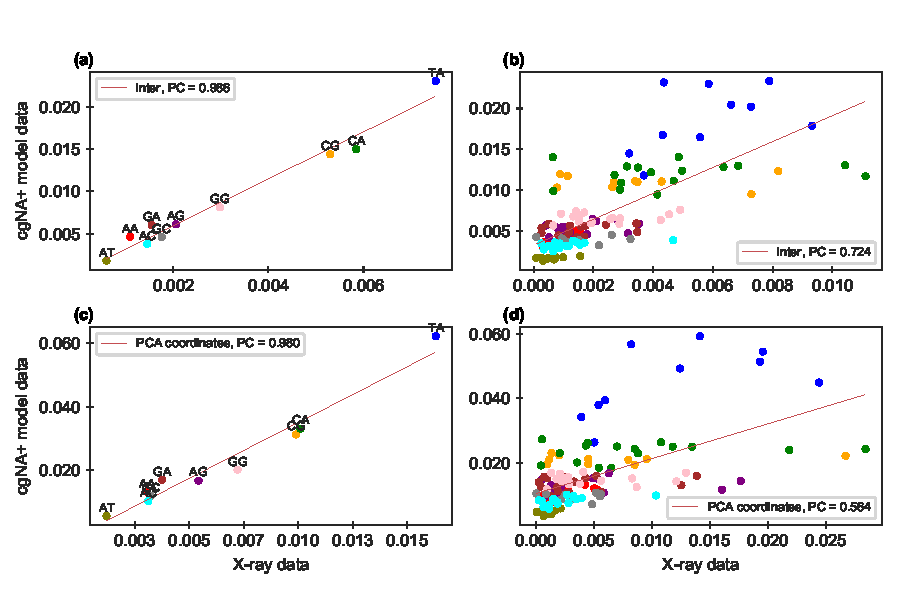
\includegraphics[trim = 0cm 0.4cm 0cm 0cm]{./Xray_images/vol_R2_DX3_3S_C1_cg.pdf}
	\centering\caption{Comparison of configurational volume
	for cgNA$+$ model covariance vs X-ray data set covariance a) in inter coordinates for independent dimer steps in average context, b) in inter coordinates for dimers in independent tetramer contexts, c) in PCA coordinates (in  eight principal modes of cgNA$+$ model shape covariance $\in \R^{18}$) for independent dimer steps in average context, d) in PCA coordinates (in  eight principal modes of cgNA$+$ model shape covariance $\in \R^{18}$) for dimers in independent tetramer contexts.
The red line is best-fit line between the two data sets using linear regression.
}

\label{fig:TX3stiff}
\end{center}
\end{figure}

We have carried out this comparison computing S\textsubscript{inter} (for inter coordinates, taking marginal over intra coordinates) and S\textsubscript{PCA8} (for the transformed coordinates in the eight principal modes of cgNA$+$ shape covariance matrix). 
For S\textsubscript{inter}, first we compared the two data sets at dimer level (i.e., average flanking context) in \cref{fig:TX3stiff}a and found an excellent correlation ($\text{PC} = 0.98$) between the two data sets.
We also observed that the YR step is significantly more flexible in inter variables than other dimer steps.
TA being the most flexible and AT most stiff (for inters parameters), which was also observed previously~\cite{lankavs2003dna, olson2006dna,el1997conformational}.
In \cref{fig:TX3stiff}b), we have compared  S\textsubscript{inter} for independent dimer in tetramer context and found good agreement (with $\text{PC} = 0.72$).
In the plot, each dimer is color-coded differently with the label described in the \cref{fig:TX3stiff}b.
S highly depends on the tetramer context for some dimers, while for others, the flanking context has a negligible effect.
In general, dimer steps that are easily deformable than the stiff ones are more sensitive to the flanking tetramer context.
For example, the most flexible YR steps (TA, CA, and CG) show a higher variation in configuration volume than RR and RY steps over the tetramer context in both data sets. 

For S\textsubscript{PCA8}, PC in the two data sets is 0.98 for dimers in average context, while for dimer in tetramer context, the PC in S\textsubscript{PCA8} for the two data sets is 0.564 as shown in \cref{fig:TX3stiff}. 
Again, we observed that soft dimers are more affected by the change in the tetramer context. 
Note that we obtained similar results on carrying out comparison in $8 \pm 2$ principal components.
We would like to highlight that the comparison of S\textsubscript{PCA8} or S\textsubscript{inter} for dimer in tetramer context is limited by the scarcity of experimental data, which might be a reason for a poor correlation.

Lastly, in \cref{SIfig:MDstiff}, we have put an analogous comparison for the cgNA$+$ model data set and MD data set. For dimer in the average context, we found PC of 0.998 for S\textsubscript{inter} and 0.998 for S\textsubscript{PCA8}. 
For dimer in tetramer context, the observed PC for S\textsubscript{inter} is 0.918 and for S\textsubscript{PCA8} is 0.922. 
%%%%%%%%%%%%%%%%%%%%%%%%%%%%%%%%%%%%%%%%%%%%%%%%%%%%%%%%%%%%%%%
%\begin{figure}[htb!]
%	\begin{center}
%	\centering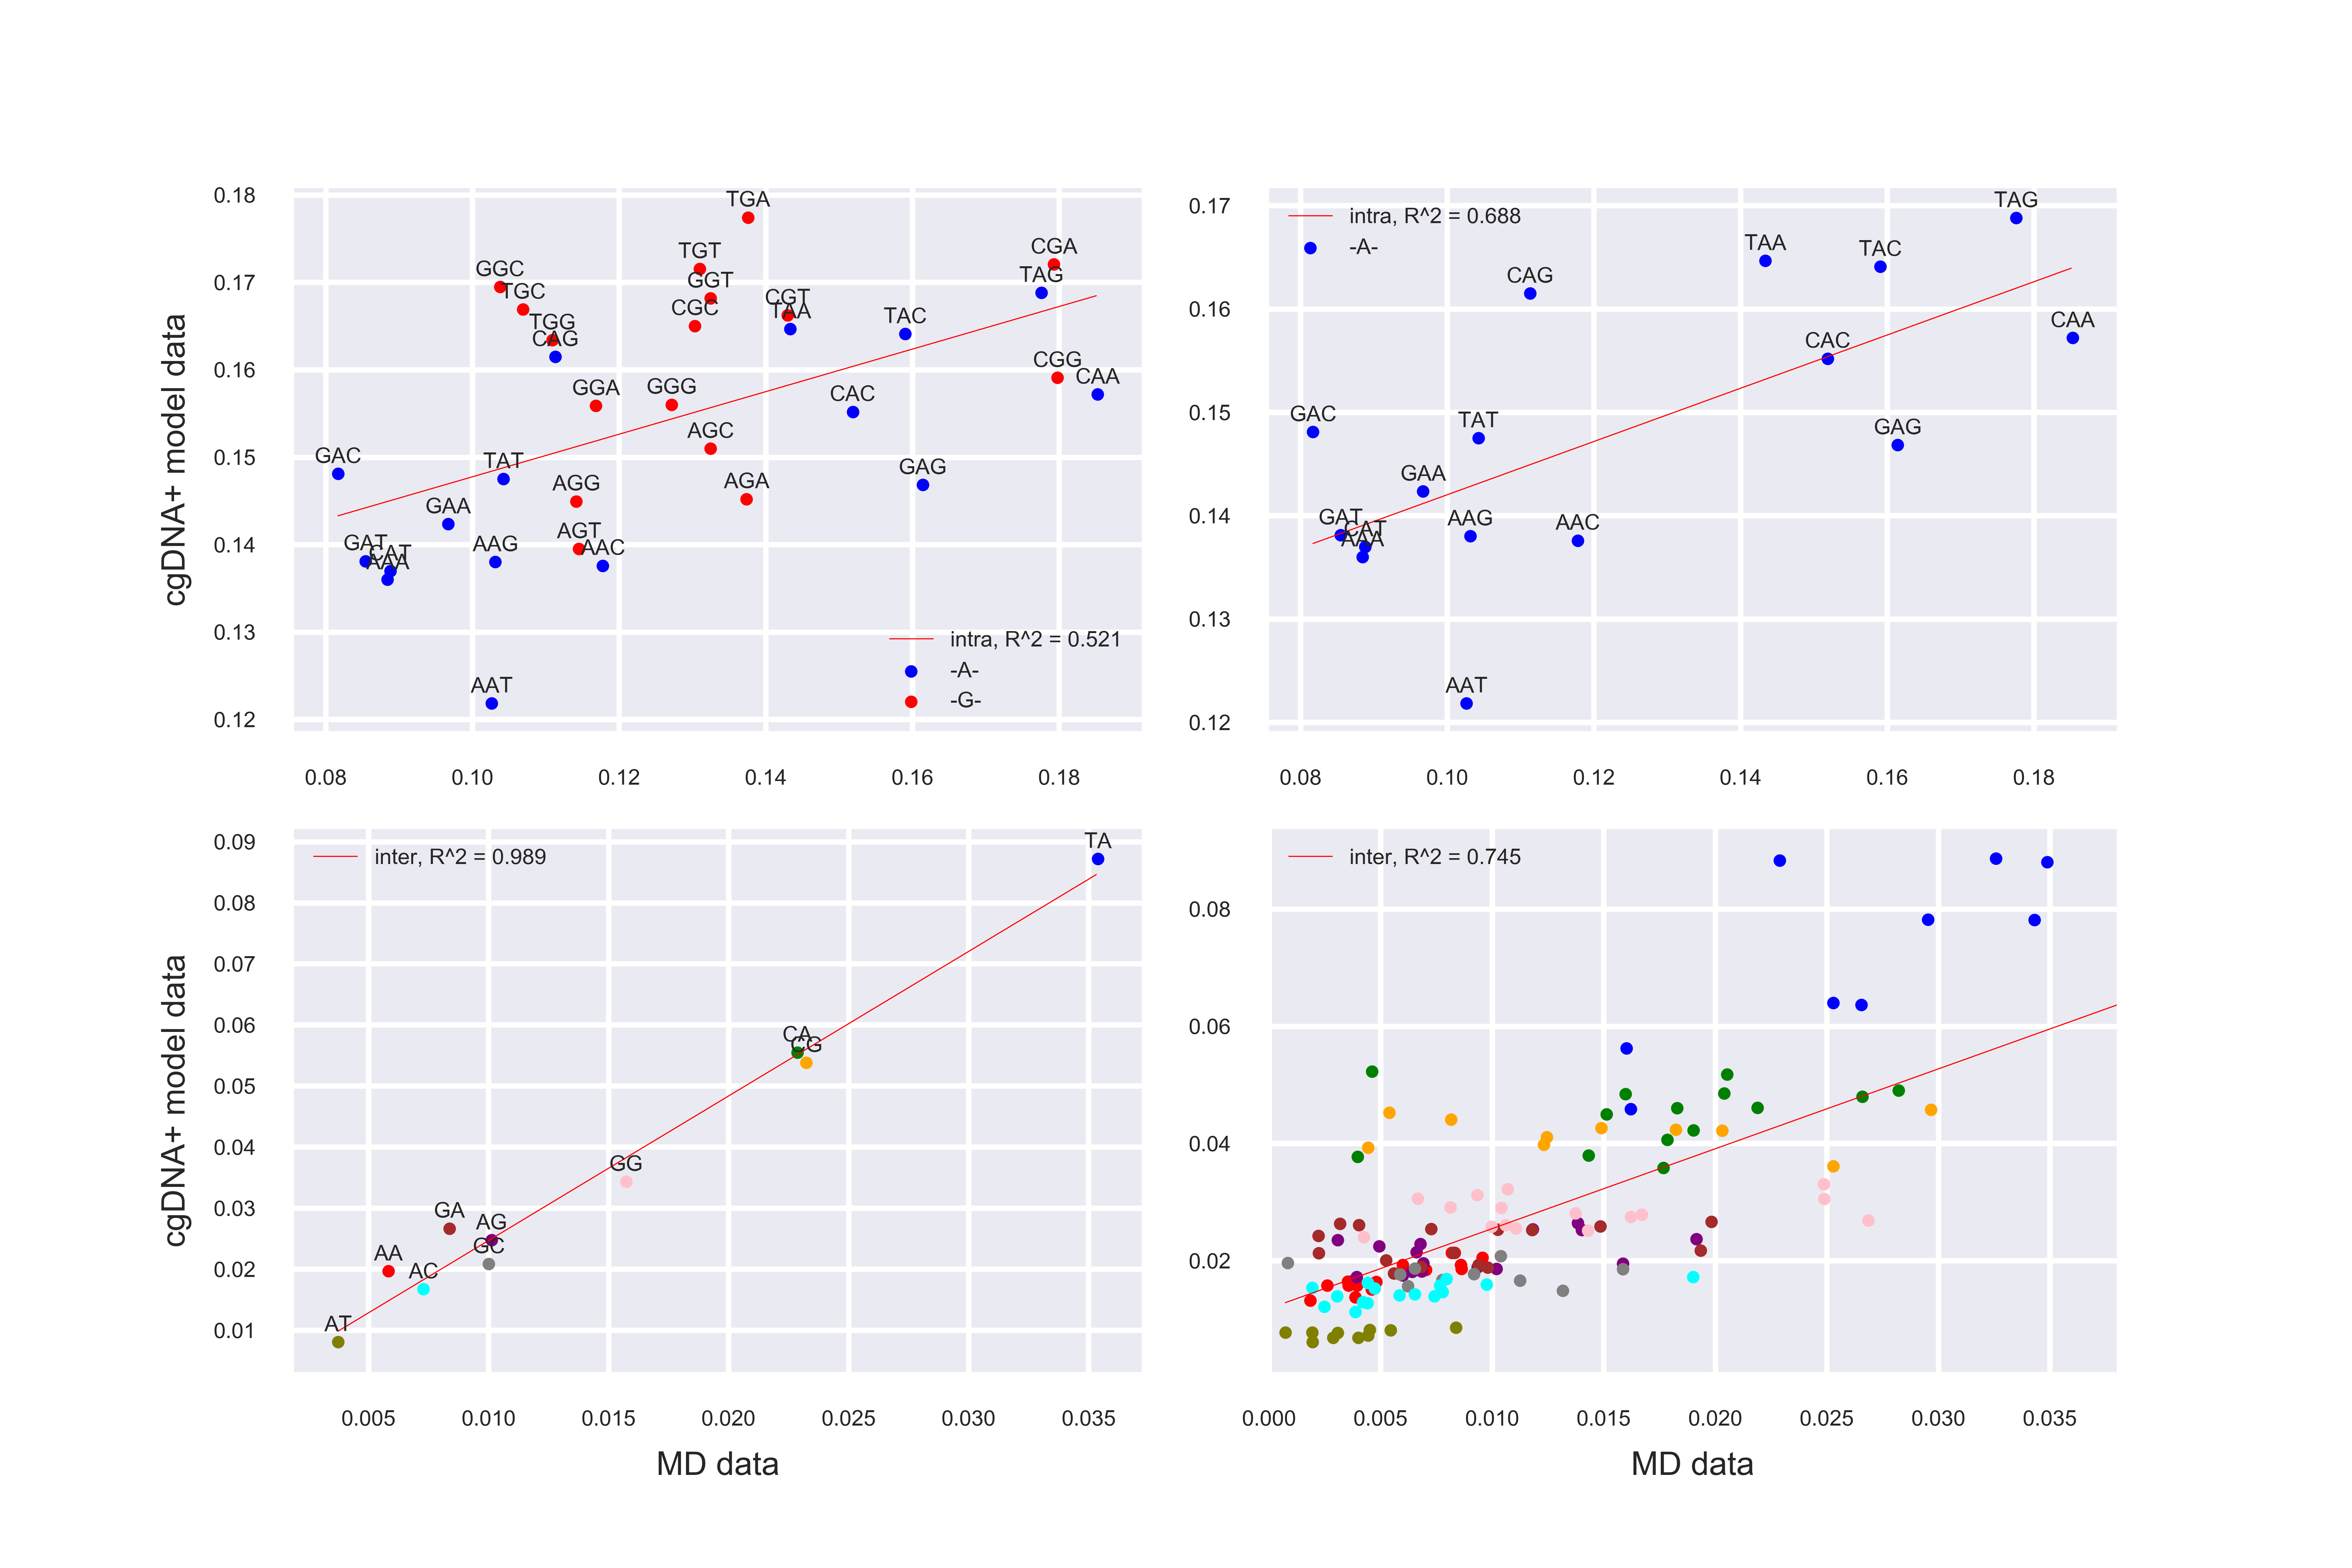
\includegraphics[scale=1]{./Xray_images/vol_R2_DX3_3S_C1_cg_sd.png}
%	\centering\caption{Comparison of configurational volume
%	for cgNA$+$ model covariance vs X-ray data covariance a) in intra coordinates for middle base-pair in independent trimer contexts, b) in intra coordinate  for A-T as the middle base-pair in trimer context, c) in inter coordinates for independent dimer steps in average context, and d) in inter coordinates for independent dimers in independent tetramer context. Note that the unit of S can be assumed \AA$^{N/2}\cdot(rad/5)^{N/2}$.
%	\red{this figure is using only sequence dominant coordinates}}
%\label{fig:TX3stiff}
%\end{center}
%\end{figure}

\section{Conclusions}
In this chapter, we have shown that cgNA$+$ model prediction is in reasonable agreement with the available protein-DNA X-ray structure database for all dimers in various tetramer contexts.
As dimer steps in the X-ray data set are often present in various flanking sequence contexts and as shown previously (in \cref{c4:figure1_rna}) that beyond tetramer flanking context could have a considerable effect on the average shape, we argued that the cgNA$+$ model is a better alternative over the MD simulations for such comparisons due to its accuracy and efficiency, which allowed computing the average shape of dimer in various tetramer contexts by averaging over all possible beyond flanking tetramer contexts.
Moreover, we have compared both intra base-pair and inter base-pair step coordinates in the two data sets. 
Notably, the comparison of the intra base-pair coordinates and for all dimers in all tetramer contexts are complete novelties.

Firstly, we have shown that the sequence-independent (or sequence-average) average shape in the two data sets is extremely close. 
Moreover, defining \say{shape covariance} as the variation of groundstate in sequence space, we have shown that the direction of variation of groundstate in sequence space, i.e., the eigenvectors of shape covariance align closely with a cosine similarity of $0.81 \pm 0.11$.
Then, we have demonstrated that, in the X-ray data, along with the central dimer step immediate tetramer flanking context is crucial in determining the average shape of dimer and in some cases, change in average shape can be larger due to change in tetramer contexts than change in central dimer step.
Also, we found that certain flanking contexts systematically influence the average shape of dimer more than others. 
Furthermore, we have also emphasized the role of sequence by performing hierarchical clustering on the average shape of dimer in tetramer contexts, resulting in four main clusters based on pyrimidine-purine steps of the central base-pair step further sub-clusters based on the specific base-pair steps. 
Notably, the results are reasonably similar in the two data sets. 

The next part of this chapter is dedicated to directly comparing internal coordinates in the two data sets.
Firstly, we found that the Pearson correlation between the two data sets for some internal coordinates is excellent; whereas the correlation is poor for a few other coordinates, such as Rise or Stretch.
We observed that coordinates with poor correlation are the ones that change the least in the sequence space, which leads to the hypothesis that for such coordinates, inherent noise in the X-ray data might have a dominating effect and, thus, it is not possible to resolve the sequence effect, in particular, the role of tetramer flanking context.
We justified this hypothesis by demonstrating that correlation for the transformed coordinates in the principal modes of shape covariance is excellent, in contrast, to the correlation in the lower modes.
Furthermore, we have also shown that Mahalanobis distance between the average shape for dimers in tetramer contexts in the two data sets is also close, however, it is not always possible to resolve dimers in various tetramer contexts.

In the final part, we have defined sequence-average \say{configuration covariance} which tells dsDNA deformation in the configuration space and found as excellent alignment (cosine similarity of $0.88 \pm 0.07$) in the eigenvectors of the configuration covariance, i.e., the direction of deformation of the two data sets.
However, the magnitude of the deformation is significantly less in the X-ray data set, which can be attributed to its lower effective temperature.
More interestingly, the directions of deformation in configuration space align well to the direction of variation in the average shape in sequence space, implying that a given dimer attains minimum total nearest-neighbor junction energies, i.e., equilibrium shape by negotiating more in the direction of soft modes.
Furthermore, for sequence-dependent analysis of dsDNA deformability, we have used the configurational volume as a metric to quantify deformability and found an excellent correlation of 0.98 at dimer level for both inter-variables and PCA coordinates (transformed on eight principal modes).
Notably, at the tetramer level, the correlation in the data set is not equally good with a Pearson correlation of 0.72 for inter-coordinates and 0.56 for PCA coordinates but are still reasonable given the scarcity of the X-ray data for dimers in various tetramer flanking contexts. 
Moreover, we found that the sensitivity in deformability to flanking contexts is maximum in flexible dimer steps (YR).

Thus, we have demonstrated that the flanking tetramer contexts are crucial for dsDNA mechanics in X-ray data, and cgNA$+$ model predictions are in reasonable agreement for both the average shape and deformability; thus, it presents itself as an excellent tool for routine investigation of non-local sequence-dependent dsDNA mechanics for various applications.

